\chapter{Experiments}
\label{ch:experiments}

This section presents experimental results regarding the
approaches to shape completion discussed in Chapter \ref{ch:shape-inference}
on all datasets introduced in Chapter \ref{ch:data}. Not all of the discussed
formulations perform equally well. Originally, we first conducted experiments
on our synthetic 2D rectangle dataset, see Appendix \ref{ch:appendix-experiments}, 
and found that maximum likelihood (\ML), does not perform well. For clarity, we
only present experiments on our synthetic 3D datasets, \ie cuboids and cars from ShapeNet
\cite{ChangFunkhouserGuibasSavarese:2015}, as well as on real data, \ie 
KITTI \cite{GeigerLenzUrtasun:2012,GeigerLenzStillerUrtasun:2013}.
Overall, we consider variational auto encoders (\VAEs) for learning shape priors
and amortized maximum likelihood (\AML) as well as
extended variational auto-encoders (\EVAEs) for shape completion.
Due to space constraints, the presented experiments are complemented
by additional results in Appendix \ref{ch:appendix-experiments}.
We first discuss the experimental setup before discussing experiments
on 3D cuboids and cars as well as on KITTI.

\section{Experimental Setup}

% TODO early stopping
% TODO training
We implemented all discussed approaches in the Torch\footnote{
  \url{http://torch.ch/}.
} deep learning framework. The implementations can be understood as prototypes;
we did not optimize them with respect to runtime or memory consumption.
Data pre-processing and generation as well as evaluation was performed in Python
and C++ as described in Chapter \ref{ch:data}. For all experiments we use a resolution
of $H \times W \times D = 32^3$ and assume a uniform subdivision of $[0,1]$ into
$32^3$ voxels for voxelization. As already stated, we derive signed distance functions
from the corresponding occupancy grids using distance transforms. Details on the
artificially added noise as well as data augmentation is discussed in the corresponding
sections.
In the following we briefly describe the used architectures
and evaluation metrics.

\subsection{Architecture and Training}

The architectures used for our experiments are kept simple.
While we experimented with deeper and more complex architectures
including skip connections, residual units \cite{HeSun:2016} and
inception-based architectures \cite{SzegedyRabinovich:2015,SzegedyWojna:2016},
these changes had no significant influence.
We follow the architectures illustrated in Figures \ref{subfig:experiments-2d-architecture-vae}
and \ref{fig:shape-inference-evae} for \VAEs and \EVAEs, respectively.
Encoder and decoder both consist of four stages of convolutional
layers including batch normalization, $\ReLU$ non-linearity and max
pooling/nearest neighbor upsampling. We follow discussions
in the literature \cite{SzegedyWojna:2016}
and increase the width of the network (\ie the number of channels) whenever decreasing the
spatial size of the feature maps and use $3 \times 3 \times 3$ convolution kernels
with zero padding and non-overlapping $2 \times 2 \times 2$ windows for max pooling and
nearest neighbor upsampling. For $32 \times 32 \times 32$ we thus reduce the spatial
size to $2 \times 2 \times 2$ before computing the latent code.
For both \AML and \EVAE, the new encoders, \ie $z(x; w)$ and $q(z | x)$, are trained from
scratch but follow the architecture of the shape prior. In this case, the corresponding
generative model $p(y | z)$ is always kept fixed.
For \AML, we additionally remove the fully connected layer predicting
the variance of the latent code
to obtain a deterministic encoder. For \EVAE, the additional decoder $p(x | y)$
consists of seven convolutional stages including batch normalization and
$\ReLU$ non-linearities. When predicting occupancy, we use Sigmoid non-linearities;
for predicting signed distance functions we use the identity, \ie no non-linearity.
We refer to Appendix \ref{ch:appendix-experiments} for training details.

\subsection{Evaluation}
\label{sec:experiments-2d-evaluation}

For evaluation we resort to the absolute error between prediction
and ground truth for both representations, \ie occupancy and signed distance functions.
For a prediction
$y \in \mathbb{R}^{H \times W \times D}$ and ground truth
$y^* \in \mathbb{R}^{H \times W \times D}$ we average over all spatial dimensions:
\begin{align}
  \Abs(y, y^*) = \frac{1}{HWD} \sum_{i_1 = 1}^H \sum_{i_2 = 1}^W \sum_{i_3 = 1}^D \left|y_i - y^*_i\right|.
  \label{eq:experiments-2d-abs}
\end{align}
We always report the average on the validation set (or on batches during training).
We additionally use the absolute error after thresholding the predicted shapes,
\ie after obtaining proper occupancy grids. For occupancy grids, we threshold 
the predicted occupancy probabilities at $0.5$ and
for signed distance functions we threshold at $0$ (here, negative values correspond
to occupied voxels). These thresholds are also used for our 3D visualizations.
We refer to the absolute error after thresholding as $\AbsThr$. Overall,
the absolute error is easy to interpret,
\eg it provides a clear lower bound (which is $\Abs \geq 0$), and comparable
across datasets and methods.

Because the discussed approaches try to maximize the likelihood -- or the
corresponding evidence lower bound -- during training, we would also like
to consider the negative log-likelihood as measure.
However, we found the negative log-likelihood to be unsuited for evaluation.
First, the negative log-likelihood is harder to interpret as it strongly
depends on the model (\eg \VAE or \EVAE). In particular, besides the
reconstruction loss, all models also include (possibly weighted) prior terms
-- \eg in form of Kullback-Leibler divergences or the negative log-likelihood
corresponding to the prior $p(z)$. Furthermore, for \EVAE, the reconstruction loss does not
represent the objective we are actually trying to optimize for shape completion.
Second, across datasets, the negative log-likelihood depends on the number of
observed voxels. Thus, performance of the proposed shape completion approaches
cannot be compared to the reconstruction performance of the shape prior -- 
which would be a natural baseline.
Third, the negative log-likelihood on Bernoulli observations is inherently skewed
towards ``unsure'' predictions; meaning that the negative log-likelihood
prefers unsure predictions over very certain predictions with few mistakes
(see Appendix \ref{ch:appendix-experiments} for an example). This is
reasonable during training where we explicitly want to model uncertainty,
but hinders fair evaluation. Overall, we decided not to report any negative log-likelihoods.

\section{3D Example}
\label{sec:experiments-3d}

% TODO nicer tables
\begin{table}
  \centering
  {\footnotesize
  \renewcommand{\arraystretch}{1.1}
  \begin{tabularx}{\textwidth}{| X | c | c | c |}
    \hline
    & \Cub\easy & \Cub\moderate & \Cub\hard\\\hline
    Training Size (Prior/Inference) & \multicolumn{3}{c|}{$10000/10000$}\\\hline
    Validation Size & \multicolumn{3}{c|}{$1000$}\\\hline
    Resolution $H \times W \times D$ & \multicolumn{3}{c|}{$32 \times 32 \times 32$}\\\hline
    Resolution $2u \times 2v$ & $48 \times 64$ & \multicolumn{2}{c|}{$24 \times 32$}\\\hline
    Noise $\lambda_{\text{hit}}$ & $0$ & $50$ & $50$\\\hline
    Noise $\theta_{\text{ignore}}$ & $0$ & $0$ & $0.1$\\\hline
    Observed Voxels (Inference Training Set) & $1.43\%$ & $0.53\%$ & $0.48\%$\\\hline
    Free Space Voxels (Inference Training Set) & $10.73\%$ & $7.07\%$ & $8.32\%$\\\hline
    Occupied Voxels (Inference Training Set) & $16.24\%$ & $16.17\%$ & $16.21\%$\\\hline
  \end{tabularx}
  }
  \vskip 6px
  % TODO short caption
  \caption{Overview of the generated datasets. We created datasets of three
  difficulties, \easy, \moderate and \hard, which refer to increased noise
  and less observations. Details on the parameters are discussed
  in Section \ref{sec:data-3d}. Additionally, we report statistics such as the
  percentage of observed voxels, free space voxels and occupied voxels
  (of the ground truth shapes) over the training set used for shape inference.}
  \label{table:experiments-3d-datasets}
\end{table}

We start with experiments on our synthetic 3D cuboids dataset.
Here, we are able to present both quantitative and qualitative results
on a controlled, simple dataset. To this end, we created datasets of three difficulties
following the procedure in Chapter \ref{ch:data}:
\easy, \hard and \moderate with details in Table \ref{table:experiments-3d-datasets}.
With rising difficulty, less observations are provided and the underlying noise increases.
The \hard case is supposed to represent real conditions as found on KITTI.
Examples for all three difficulties can be found in Appendix \ref{ch:data}. In
Table \ref{table:experiments-3d-datasets} we additionally report some
basic statistics, \eg the percentage of occupied voxels to give an impression
of how trivial predictions would perform or the percentage of observed
and free space voxels to indicate what level of supervision is available.
We start with discussing the \VAE shape prior before proceeding to the problem
of shape completion. As we found \ML to perform poorly in the 2D case,
we exclude experiments on 3D data.

\subsection{Shape Prior}

\begin{figure}[t]
  \begin{subfigure}[t]{0.48\textwidth}
    \begin{tikzpicture}
      \begin{axis}[
          % https://tex.stackexchange.com/questions/68577/compiling-a-document-with-pgfplots-processing-only-every-x-th-data-point
          each nth point=2,
          filter discard warning=false,
          unbounded coords=discard,
          % https://tex.stackexchange.com/questions/13816/dimension-too-large-while-plotting-with-pgfplots
          %restrict y to domain=0:0.1,
          %restrict x to domain=0:250000,
          log ticks with fixed point,
          ymin=0,
          ymax=0.06,
          xmin=0,
          xmax=125000,
          %xticklabel={
          %  \pgfmathparse{\tick/1000}
          %  \pgfmathprintnumber{\pgfmathresult}k
          %},
          xtick={0,50000,100000},
          xticklabels={0,50k,100k},
          xticklabel style={
            /pgf/number format/fixed
          },
          scaled x ticks=false,
          yticklabel style={
            /pgf/number format/fixed
          },
          scaled y ticks=false,
          %x coord trafo/.code={\pgfmathparse{\pgfmathresult/1000}},
          %xticklabel=\pgfmathprintnumber{\tick}k,
          width=7.5cm,
          height=5cm,
          % https://tex.stackexchange.com/questions/48620/pgfplots-alignment-and-size-of-math-in-legend
          legend cell align=left,
        ]
        
        % https://tex.stackexchange.com/questions/276869/reading-an-unusual-coordinates-file-in-pgfplots
        \addplot +[mark=none] table[ignore chars={(,)},col sep=comma] {data/experiments/3d/vae_occ/easy_15/training_loss.txt};
        \addlegendentry{$\mathcal{L}_{\text{BCE}} + \KL$ (train)};
        \addplot +[mark=none] table[ignore chars={(,)},col sep=comma] {data/experiments/3d/vae_occ/easy_15/training_abs.txt};
        \addlegendentry{$\Abs$ (train)};
        
        \addplot +[mark=none] table[ignore chars={(,)},col sep=comma] {data/experiments/3d/vae_occ/easy_15/validation_loss.txt};
        \addlegendentry{$\mathcal{L}_{\text{BCE}} + \KL$ (val)};
        \addplot +[mark=none] table[ignore chars={(,)},col sep=comma] {data/experiments/3d/vae_occ/easy_15/validation_abs.txt};
        \addlegendentry{$\Abs$ (val)};
      \end{axis}
    \end{tikzpicture}
  \end{subfigure}\hfill
  \begin{subfigure}[t]{0.48\textwidth}
    \begin{tikzpicture}
      \begin{axis}[
          % https://tex.stackexchange.com/questions/68577/compiling-a-document-with-pgfplots-processing-only-every-x-th-data-point
          %each nth point=100,
          filter discard warning=false,
          unbounded coords=discard,
          % https://tex.stackexchange.com/questions/13816/dimension-too-large-while-plotting-with-pgfplots
          %restrict y to domain=0:0.1,
          %restrict x to domain=0:250000,
          %ymin=0,
          %ymax=0.4,
          xmin=0,
          xmax=125000,
          %xticklabel={
          %  \pgfmathparse{\tick/1000}
          %  \pgfmathprintnumber{\pgfmathresult}k
          %},
          xtick={0,50000,100000},
          xticklabels={0,50k,100k},
          xticklabel style={
            /pgf/number format/fixed
          },
          scaled x ticks=false,
          yticklabel style={
            /pgf/number format/fixed
          },
          scaled y ticks=false,
          %x coord trafo/.code={\pgfmathparse{\pgfmathresult/1000}},
          %xticklabel=\pgfmathprintnumber{\tick}k,
          width=7.5cm,
          height=5cm,
          % https://tex.stackexchange.com/questions/48620/pgfplots-alignment-and-size-of-math-in-legend
          legend cell align=left,
        ]
        
        \addplot +[mark=none] table[ignore chars={(,)},col sep=comma] {data/experiments/3d/vae_occ/easy_15/validation_mean.txt};
        \addlegendentry{$\overline{\mu}$ (val)};
        \addplot +[mark=none] table[ignore chars={(,)},col sep=comma] {data/experiments/3d/vae_occ/easy_15/validation_var.txt};
        \addlegendentry{$\exp\left(\frac{1}{2}\overline{l}\right)$ (val)};
        \addplot +[mark=none] table[ignore chars={(,)},col sep=comma] {data/experiments/3d/vae_occ/easy_15/validation_std.txt};
        \addlegendentry{$|1 - \sqrt{\Var[\mu]}|$ (val)};
      \end{axis}
    \end{tikzpicture}
  \end{subfigure}
  \caption{Training curves for a \VAE with $Q = 15$ trained on the 3D cuboids dataset. We show
  the training loss, \ie $\mathcal{L}_{\text{BCE}} + \KL$, on the training (train) and validation set (val)
  as well as the corresponding absolute error \Abs on the left. Statistics corresponding to the latent
  space, particularly, the average $\overline{\mu}$ of the predicted means and the corresponding 
  standard deviation $\sqrt{\Var[\mu]}$ as well as the average of the predicted standard
  deviations $\exp(\frac{1}{2} \overline{l})$ are shown on the right. For the latter we also
  refer to Equations \eqref{eq:shape-prior-monitor-mean-mean}, \eqref{eq:shape-prior-monitor-variance-mean}
  and \eqref{eq:shape-prior-monitor-mean-variance} for details.}
  \label{fig:experiments-3d-vae-t}
\end{figure}

\begin{figure}
  \centering
  \vspace{-0.25cm}
  \begin{tikzpicture}
    \node at (0, 1.1){
      \includegraphics[width=6cm]{experiments/3d/vae_occ/easy_15/results_0}
    };
    \node at (0, -1.1){
      \includegraphics[width=6cm]{experiments/3d/vae_occ/easy_15/results_1}
    };
    
    \draw[-,dashed] (3.25, -8) -- (3.25,3);
    
    \node at (6.5, 0){
      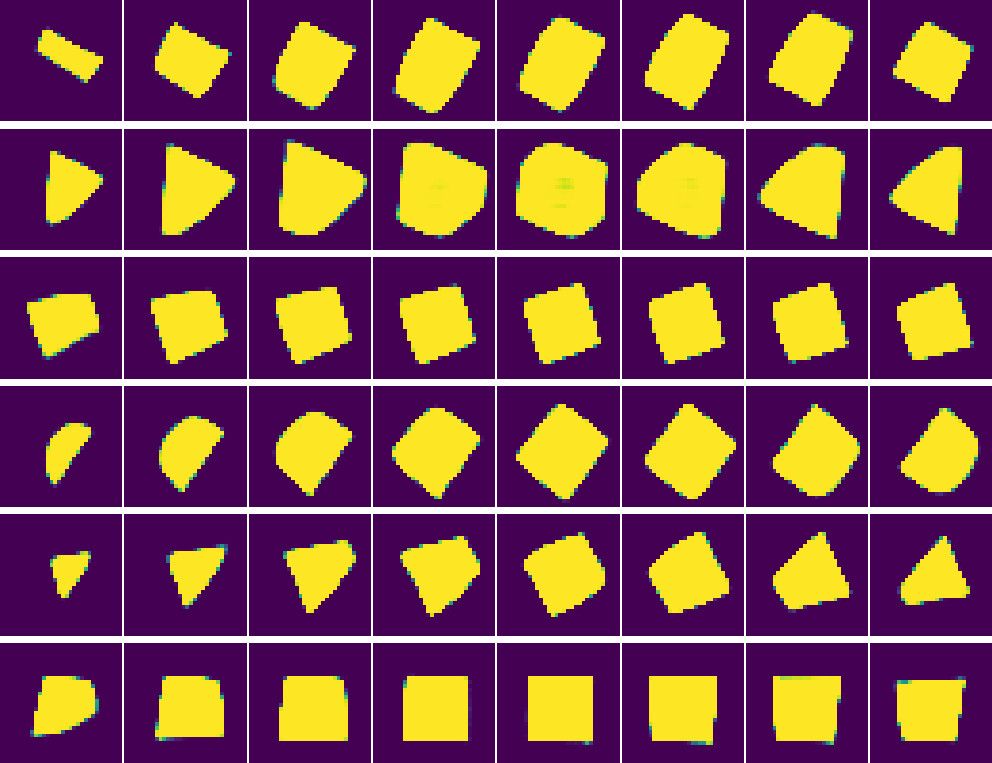
\includegraphics[width=6cm]{experiments/3d/vae_occ/easy_15/random}
    };
    
    \node at (10,0) {
      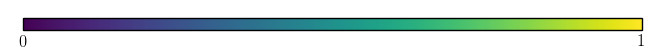
\includegraphics[height=5cm]{experiments/3d/vae_occ/easy_15/colorbar}
    };
    
    \node at (0, 3) {\begin{tabular}{c}reconstruction\\occupancy\end{tabular}};
    \node at (6.5, 3) {\begin{tabular}{c}random samples\\occupancy\end{tabular}};
    
    \draw[-,dashed] (-3.5, -2.5) -- (10, -2.5);
    
    %\node at (-3.5,-5) {
    %  \includegraphics[height=5cm]{experiments/3d/vae_occ_sdf/colorbar_0}
    %};
    
    \node at (0, -5){
      \includegraphics[width=6cm]{experiments/3d/vae_occ_sdf/easy_15/random_0_0}
    };
    
    %\draw[-,dashed] (3.25, -3) -- (3.25,3);
    
    \node at (6.5, -5){
      \includegraphics[width=6cm]{experiments/3d/vae_occ_sdf/easy_15/random_0_1}
    };
    
    \node at (10,-5) {
      \includegraphics[height=5cm]{experiments/3d/vae_occ_sdf/colorbar_1}
    };
   
    \node[rotate=90] at (-3.75, 0) {\begin{tabular}{c}predicting occupancy only\end{tabular}};
    \node[rotate=90] at (-3.75, -5) {\begin{tabular}{c}predicting occupancy and\\signed distance functions\end{tabular}};
   
    \node at (0, -8) {\begin{tabular}{c}random samples\\occupancy\end{tabular}};
    \node at (6.5, -8) {\begin{tabular}{c}random samples\\signed distance functions\end{tabular}};
  \end{tikzpicture}
  
  % TODO short caption
  \caption{Qualitative results for the trained \VAE shape prior with $Q = 15$ on the 3D cuboids dataset.
  We consider two models; one trained on occupancy only and one trained on both occupancy and
  signed distance functions. In the first case, we show reconstruction results on the left and
  random samples on the right. For the latter case, we show only random samples for both modalities.
  In all cases we show horizontal slices, \ie heights $8 + 2i$ for $0 \leq i < 8$. For random samples
  in the occupancy only case, we complement the results with 3D visualizations in Figure
  \ref{fig:experiments-3d-vae-qual-2}.}
  \label{fig:experiments-3d-vae-qual-1}
\end{figure}
\begin{figure}
  \centering
  \vspace{-0.25cm}
  \hspace*{-1cm}
  \begin{tikzpicture}
    \node at (0, 0) {
      \includegraphics[width=2.5cm,trim={2cm 1cm 2cm 1cm},clip]{experiments/3d/vae_occ/easy_15/0_random_15}
    };
    \node at (2.5, 0) {
      \includegraphics[width=2.5cm,trim={2cm 1cm 2cm 1cm},clip]{experiments/3d/vae_occ/easy_15/0_random_105}
    };
    
    \draw[-,dashed] (4,-1.5) -- (4, 1.5);
    
    \node at (5.5, 0) {
      \includegraphics[width=2.5cm,trim={2cm 1cm 2cm 1cm},clip]{experiments/3d/vae_occ/easy_15/5_random_15}
    };
    \node at (8, 0) {
      \includegraphics[width=2.5cm,trim={2cm 1cm 2cm 1cm},clip]{experiments/3d/vae_occ/easy_15/5_random_105}
    };
    
    \draw[-,dashed] (9.5,-1.5) -- (9.5, 1.5);
    
    \node at (11, 0) {
      \includegraphics[width=2.5cm,trim={2cm 1cm 2cm 1cm},clip]{experiments/3d/vae_occ/easy_15/2_random_15}
    };
    \node at (13.5, 0) {
      \includegraphics[width=2.5cm,trim={2cm 1cm 2cm 1cm},clip]{experiments/3d/vae_occ/easy_15/2_random_105}
    };
  \end{tikzpicture}
  \caption{Three random example of the \VAE shape prior with $Q = 15$ on the 3D cuboids dataset
  trained on occupancy only. In all three cases, we show two different viewpoints. We find that all
  three examples resemble cuboids. We also note that the \VAE has no difficulties predicting sharp corners
  and edges.}
  \label{fig:experiments-3d-vae-qual-2}
\end{figure}


For the shape prior, the size $Q$ of the latent space is crucial. We found that in
practice a suitable size can be determined by monitoring the training progress
of the \VAE for different sizes $Q$. For the following discussion, we determined
$Q = 15$ to be suitable and the corresponding training curves are shown
in Figure \ref{fig:experiments-3d-vae-t}.
%A comparison to $Q = 5$ and $Q = 30$ can be found in the appendix.
An important cue to judge $Q$
is the latent space, \ie whether learning the latent space converged. This is
usually be indicated by low predicted log-variances and the statistics of the predicted
means slowly resembling a unit Gaussian (\ie zero mean and unit variance).
Additionally, the obtained reconstruction error can be used as indicator. For $Q = 5$,
for example, the absolute error does not fall below $ \Abs \approx 0.04$.
Considering that, only
$~16.2\%$ of the voxels are occupied (\cf Table \ref{table:experiments-3d-datasets})
this error is still
very large. For $Q = 15$ and above, in contrast, the error reduces to $\Abs \approx 0.0054$ or lower.
Finally, we also consider random samples utilizing the generative model.
As can be seen in Figures \ref{fig:experiments-3d-vae-qual-1}
and \ref{fig:experiments-3d-vae-qual-2}, the random samples
look appropriate and mostly resemble cuboids.
Note that due to rotations, the cuboids might not appear rectangular when
showing horizontal slices of the corresponding volumes.
Overall, we did not exploit all possibilities regarding hyper parameters and
training time, but are satisfied with the obtained performance
using $Q = 15$.

On 2D examples, we realized that predicting both occupancy and signed
distance functions is beneficial compared to predicting signed distance functions
only. On 3D, we make a similar observation and show qualitative results
in Figure \ref{fig:experiments-3d-vae-qual-1}. Again, we use $Q = 15$,
and achieve an absolute error of $\Abs \approx 0.0064$ for occupancy and
$\Abs \approx 0.071$ for signed distance functions. After thresholding the
predicted representations to obtain occupancy grids (at $0.5$ for occupancy
probabilities and at $0$ for signed distance functions), the absolute error
drops to $\AbsThr \approx 0.0045$ and $\AbsThr \approx 0.0053$, respectively.
This means that both representations can be used to derive low-error
occupancy grids. Random samples also look suitable and clearly depict cuboids in
most cases; however, we find the samples to be slightly less sharp compared to
predicting occupancy only.
%For brevity, we include further qualitative results
%as well as training curves in Appendix \ref{ch:appendix-experiments}.

\subsection{Amortized Maximum Likelihood}
\label{sec:experiments-3d-aml}

\begin{figure}
  \centering
  \begin{subfigure}[t]{0.48\textwidth}
    \begin{tikzpicture}
      \begin{axis}[
          % https://tex.stackexchange.com/questions/68577/compiling-a-document-with-pgfplots-processing-only-every-x-th-data-point
          %each nth point=2,
          filter discard warning=false,
          unbounded coords=discard,
          % https://tex.stackexchange.com/questions/13816/dimension-too-large-while-plotting-with-pgfplots
          %restrict y to domain=0:0.1,
          %restrict x to domain=0:250000,
          ymin=0,
          ymax=0.12,
          xmin=0,
          xmax=31000,
          %xticklabel={
          %  \pgfmathparse{\tick/1000}
          %  \pgfmathprintnumber{\pgfmathresult}k
          %},
          xtick={0,15000,31000},
          xticklabels={0,15k,31k},
          xticklabel style={
            /pgf/number format/fixed
          },
          scaled x ticks=false,
          yticklabel style={
            /pgf/number format/fixed
          },
          scaled y ticks=false,
          %x coord trafo/.code={\pgfmathparse{\pgfmathresult/1000}},
          %xticklabel=\pgfmathprintnumber{\tick}k,
          width=7.5cm,
          height=5cm,
          % https://tex.stackexchange.com/questions/48620/pgfplots-alignment-and-size-of-math-in-legend
          legend cell align=left,
        ]
        
        % https://tex.stackexchange.com/questions/276869/reading-an-unusual-coordinates-file-in-pgfplots
        \addplot +[mark=none] table[ignore chars={(,)},col sep=comma] {data/experiments/3d/vae_occ_aml/moderate_15/training_loss.txt};
        \addlegendentry{$\mathcal{L}_{\text{BCE}} + \KL$ (train)};
        \addplot +[mark=none] table[ignore chars={(,)},col sep=comma] {data/experiments/3d/vae_occ_aml/moderate_15/training_abs.txt};
        \addlegendentry{$\Abs$ (train)};
        
        \addplot +[mark=none] table[ignore chars={(,)},col sep=comma] {data/experiments/3d/vae_occ_aml/moderate_15/validation_loss.txt};
        \addlegendentry{$\mathcal{L}_{\text{BCE}} + \KL$ (val)};
        \addplot +[mark=none] table[ignore chars={(,)},col sep=comma] {data/experiments/3d/vae_occ_aml/moderate_15/validation_abs.txt};
        \addlegendentry{$\Abs$ (val)};
      \end{axis}
    \end{tikzpicture}
  \end{subfigure}\hfill
  \begin{subfigure}[t]{0.48\textwidth}
    \begin{tikzpicture}
      \begin{axis}[
          % https://tex.stackexchange.com/questions/68577/compiling-a-document-with-pgfplots-processing-only-every-x-th-data-point
          %each nth point=100,
          filter discard warning=false,
          unbounded coords=discard,
          % https://tex.stackexchange.com/questions/13816/dimension-too-large-while-plotting-with-pgfplots
          %restrict y to domain=0:0.1,
          %restrict x to domain=0:250000,
          ymin=-0.2,
          ymax=0.5,
          xmin=0,
          xmax=31000,
          %xticklabel={
          %  \pgfmathparse{\tick/1000}
          %  \pgfmathprintnumber{\pgfmathresult}k
          %},
          xtick={0,15000,31000},
          xticklabels={0,15k,31k},
          xticklabel style={
            /pgf/number format/fixed
          },
          scaled x ticks=false,
          yticklabel style={
            /pgf/number format/fixed
          },
          scaled y ticks=false,
          %x coord trafo/.code={\pgfmathparse{\pgfmathresult/1000}},
          %xticklabel=\pgfmathprintnumber{\tick}k,
          width=7.5cm,
          height=5cm,
          % https://tex.stackexchange.com/questions/48620/pgfplots-alignment-and-size-of-math-in-legend
          legend cell align=left,
        ]
        
        \addplot +[mark=none] table[ignore chars={(,)},col sep=comma] {data/experiments/3d/vae_occ_aml/moderate_15/validation_mean.txt};
        \addlegendentry{$\overline{\mu}$ (val)};
        \addplot +[mark=none] table[ignore chars={(,)},col sep=comma] {data/experiments/3d/vae_occ_aml/moderate_15/validation_std.txt};
        \addlegendentry{$|1 - \sqrt{\Var[\mu]}|$ (val)};
      \end{axis}
    \end{tikzpicture}
  \end{subfigure}
  
  % TODO short caption
  \caption{Training curves for \AML using occupancy only and a \VAE prior
  with $Q = 15$ on the 3D cuboids dataset, specifically the \moderate case.
  Again, we show the quantities as in Figure \ref{fig:experiments-3d-vae-t}.
  We want to highlight that training takes place in the first few iterations;
  afterwards, training stagnates mostly.}
  \label{fig:experiments-3d-aml-t}
\end{figure}

\begin{figure}
  \centering
  \begin{tikzpicture}
    \begin{axis}[
        ybar stacked,
        % https://tex.stackexchange.com/questions/119887/remove-the-scientific-notation-which-is-unreasonable
        yticklabel style={
          /pgf/number format/fixed,
          /pgf/number format/precision=5
        },
        scaled y ticks=false,
        %enlargelimits=0.15,
        legend style={
          at={(1.01,1)},
          anchor=north west,
        },
        % https://tex.stackexchange.com/questions/48620/pgfplots-alignment-and-size-of-math-in-legend
        legend cell align=left,
        xtick={
          1, 2,
          3, 4, 5,
          6, 7, 8,
          9, 10, 11
        },
        xticklabels={
          \VAE, \VAE occ+sdf,
          \AML\\\easy, \AML\\\moderate, \AML \\\hard,
          \EVAE\\\easy, \EVAE\\\moderate, \EVAE\\\hard,
          \AML occ+sdf\\\easy, \AML occ+sdf\\\moderate, \AML occ+sdf\\\hard
        },
        x tick label style={text width=1.5cm,align=right},
        ymin=0,
        width=12.5cm,
        height=4cm,
        % https://tex.stackexchange.com/questions/271027/pgfplots-how-to-rotate-extra-x-tick-labels
        x tick label style={
          rotate=90,
          anchor=east,
        },
        enlarge x limits=0.05,
        % https://tex.stackexchange.com/questions/47882/formatting-a-pgfplot-graph-thicker-bars-and-total-width
        %bar width=8,
      ]
        
      % AbsThr
      \addplot +[bar shift=-.2cm] coordinates {
        (1, 0.00384198)
        (2, 0.00453785)
        (3, 0.03217211)
        (4, 0.03567748)
        (5, 0.04434539)
        %
        (6, 0.03876815)
        (7, 0.05154616)
        (8, 0.07254225)
        %
        (9, 0.04437874)
        (10, 0.05507257)
        (11, 0.0500495)
      };
      \addlegendentry{\AbsThr (occ)}
      % Abs
      \addplot +[bar shift=-.2cm] coordinates {
        (1, 0.00155) % 0.00539829)
        (2, 0.001953) % 0.00649281)
        (3, 0.000155) % 0.03232507)
        (4, 0.000218) % 0.03588854)
        (5, 0.000445) % 0.04479165)
        %
        (6, 0.00072) % 0.03942102)
        (7, 0.0003) % 0.05189751)
        (8, 0.00031) % 0.07285957)
        %
        (9, 0.0002) % 0.04457945)
        (10, 0.00016) % 0.05523896)
        (11, 0.00019) % 0.05023721)
      };
      \addlegendentry{\Abs (occ)}
      
      % --
      \resetelevenstackedplots
      
      % AbsThr
      \addplot +[bar shift=+.2cm] coordinates {
        (1, 0)
        (2, 0.00534606)
        (3, 0)
        (4, 0)
        (5, 0)
        %
        (6, 0)
        (7, 0)
        (8, 0)
        %
        (9, 0.04459624)
        (10, 0.05582422)
        (11, 0.05130592)
      };
      \addlegendentry{\AbsThr (sdf)}
      % Abs
      \addplot +[bar shift=+.2cm] coordinates {
        (1, 0)
        (2, 0.06582) % 0.07112682)
        (3, 0)
        (4, 0)
        (5, 0)
        %
        (6, 0)
        (7, 0)
        (8, 0)
        %
        (9, 0.17411) % 0.21871304)
        (10, 0.21636) % 0.27216289)
        (11, 0.2225) % 0.27388566)
      };
      \addlegendentry{\Abs (sdf)}
    \end{axis}
  \end{tikzpicture}
  
  % TODO short caption
  \caption{Absolute error \Abs and its thresholded variant \AbsThr, \ie
  the absolute error on thresholded predictions,
  for a comparison between the \VAE prior, \AML and \EVAE on occupancy only
  and \AML predicting both occupancy and signed distance functions (indicated as occ+sdf).
  In each case, the left bar represents results on occupancy; the right bar
  corresponds to results on signed distance functions (if applicable). The comparison
  to the \VAE prior provides a possible lower bound on the performance.}
  \label{fig:experiments-3d-aml-abs}
\end{figure}

\begin{figure}
  \centering
  \vskip -0.25cm
  \begin{tikzpicture}    
    \node at (0, 0){
      \includegraphics[width=6cm]{experiments/3d/vae_occ_aml/moderate_15/results_0}
    };
    \node at (0, -2.75) {
      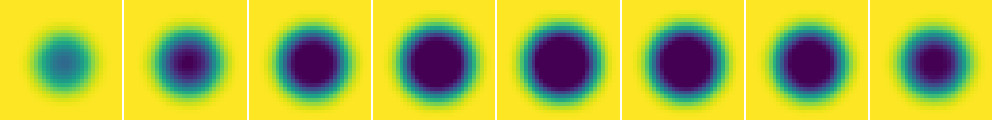
\includegraphics[width=6cm]{experiments/3d/vae_occ_aml/inference_statistics_05}
    };
    \node at (0, -5.25){
      \includegraphics[width=6cm]{experiments/3d/vae_occ_aml/hard_15_statistics_05/results_0}
    };
    \node at (0, -9.75){
      \includegraphics[width=6cm]{experiments/3d/vae_evae/hard_15_statistics/results_0}
    };
    
    %\draw[-,dashed] (3.25, -3) -- (3.25,3);
    
    \node at (6.5, 0){
      \includegraphics[width=6cm]{experiments/3d/vae_occ_aml/moderate_15/results_1}
    };
    \node at (6.5, -2.75) {
      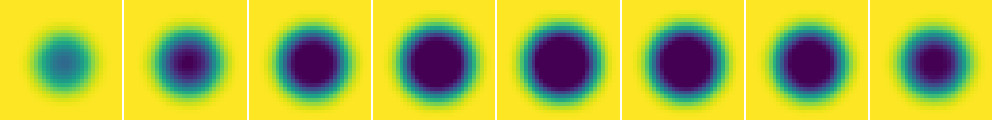
\includegraphics[width=6cm]{experiments/3d/vae_occ_aml/inference_statistics_05}
    };
    \node at (6.5, -5.25){
      \includegraphics[width=6cm]{experiments/3d/vae_occ_aml/hard_15_statistics_05/results_1}
    };
    \node at (6.5, -9.75){
      \includegraphics[width=6cm]{experiments/3d/vae_evae/hard_15_statistics/results_1}
    };
    
    \node at (10,0) {
      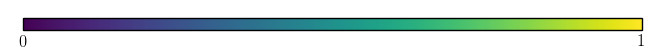
\includegraphics[height=4.25cm]{experiments/3d/vae_occ/easy_15/colorbar}
    };
   
    \draw[-,dashed] (-3.5,-2.125) -- (10,-2.125);
    \draw[-,dashed] (-3.5,-7.5) -- (10,-7.5);
    
    \node[rotate=90] at (-4, 0) {\begin{tabular}{c}\AML\\\moderate\end{tabular}};
    \node[rotate=90] at (-4, -4.25) {\begin{tabular}{c}\AML\\\hard\end{tabular}};
    \node[rotate=90] at (-4, -9.75) {\begin{tabular}{c}\EVAE\\\hard\end{tabular}};
    
  \end{tikzpicture}
  \vskip 6px
  
  % TODO short caption
  \caption{Qualitative results for \AML on the 3D cuboids dataset with a \VAE
  prior and $Q = 15$. We
  show results on \moderate and \hard difficulties in comparison with \EVAE.
  In all cases we show
  horizontal slices of the volumes, \ie heights $8 + 2i$ for $0 \leq i < 8$,
  for two samples samples,
  each showing the observed points, the partial free space, the target shape
  as well as the predicted shape and
  the corresponding error. For \AML and the hard case we additionally
  illustrate the weights $\rho_i$ that
  were used for both \AML and \EVAE.}
  \label{fig:experiments-3d-aml-qual-1}
\end{figure}
\begin{figure}
  \centering
  \vskip -0.25cm
  \begin{tikzpicture}    
    \node at (0, 0){
      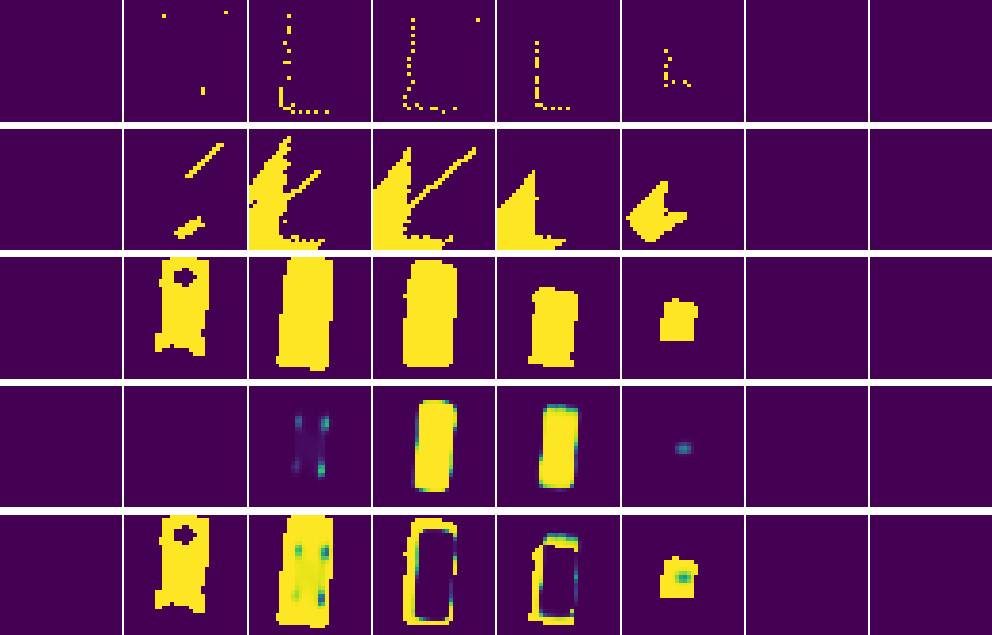
\includegraphics[width=6cm]{experiments/3d/vae_occ_sdf_aml/hard_15_statistics/results_0_0}
    };
    \node at (0, -4){
      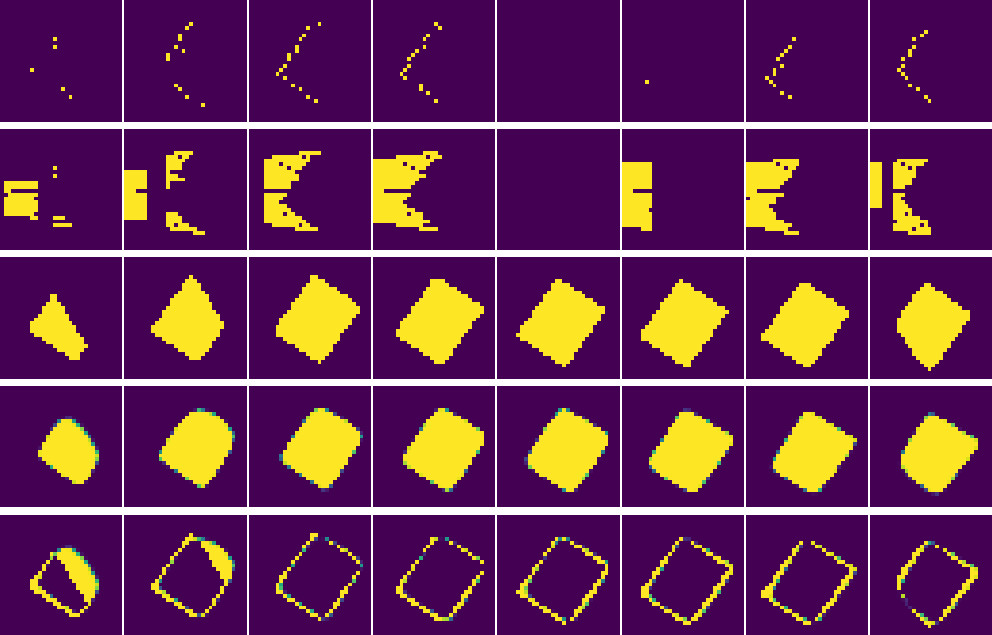
\includegraphics[width=6cm]{experiments/3d/vae_occ_sdf_aml/hard_15_statistics/results_1_0}
    };
    
    %\draw[-,dashed] (3.25, -3) -- (3.25,3);
    
    \node at (6.5, 0){
      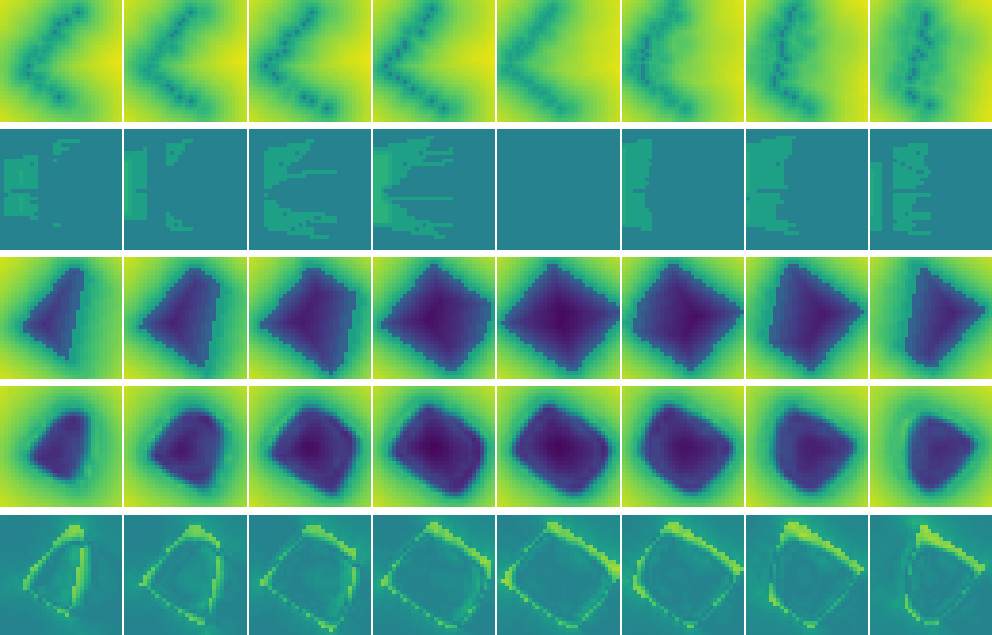
\includegraphics[width=6cm]{experiments/3d/vae_occ_sdf_aml/hard_15_statistics/results_0_1}
    };
    \node at (6.5, -4){
      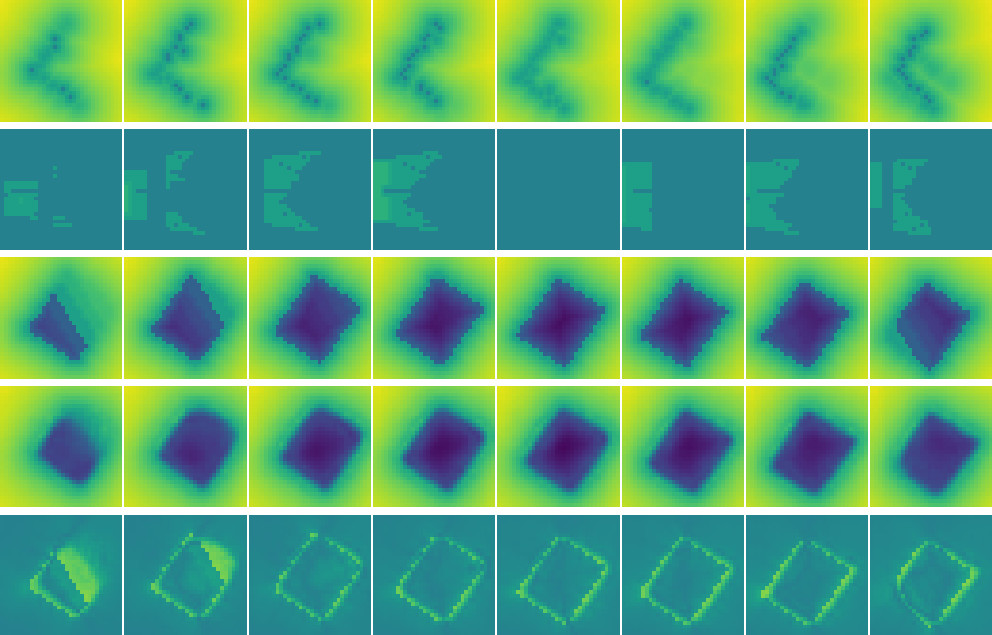
\includegraphics[width=6cm]{experiments/3d/vae_occ_sdf_aml/hard_15_statistics/results_1_1}
    };
    
    \node at (10,0) {
      \includegraphics[height=4.25cm]{experiments/3d/vae_occ_sdf_aml/colorbar_1}
    };
    
    \node at (-3.5,0) {
      \includegraphics[height=4.25cm]{experiments/3d/vae_occ_sdf_aml/colorbar_0}
    };
    
    \node at (0, 2.25) {occupancy};
    \node at (6.5, 2.25) {signed distance function};
    
  \end{tikzpicture}
  \vskip 6px
  
  % TODO short caption
  \caption{Qualitative results for \AML using a \VAE prior with $Q = 15$ trained on both
  occupancy and signed distance functions. Results correspond to the \hard case.
  We show two samples and both modalities. In all
  cases we show horizontal slices as in Figure \ref{fig:experiments-3d-aml-qual-1}
  corresponding to the observed points, the partial free space, the target shape as well as the
  predicted shape and its error. We selected two examples illustrating that 
  the model resorts to blob-like ``standard'' shapes.}
  \label{fig:experiments-3d-aml-qual-2}
\end{figure}



For \AML, we mainly present experiments on \moderate and \hard difficulties
as we found that \AML performs very well on \moderate difficulty.
%However,
%we provide additionally qualitative results for all cases in the appendix.
First of all, we note that the weight $\kappa$ on the negative log-likelihood of the prior, \ie
$- \ln p(z)$, is crucial for successful training. 
Figure \ref{fig:experiments-3d-aml-t} shows training curves for the \moderate case
when using $\kappa = 15$. Overall, the network achieves an absolute error of
$\Abs \approx 0.036$. If the weight $\kappa$ would not be large enough,
the network would quickly deviate from the unit Gaussian prior.
This can be observed
when monitoring the latent space, \ie the observed statistics $\sqrt{\Var[\mu]}$ and $\overline{\mu}$
deviate significantly from the unit Gaussian prior. If $\kappa$ is chosen too large, the prior
``collapses'', \ie $\sqrt{\Var[\mu]}$ approaches zero. If weighted
correctly, the prior takes care of enforcing the unit Gaussian in the first few iterations.
We found that matching the prior becomes important as a big portion of learning
takes place in the early iterations. This can also be seen in Figure
\ref{fig:experiments-3d-aml-t}; it seems that \AML needs only few epochs to
``learn'' inference.
Experimentally, we found that $\kappa = 15$ performs
well for the \moderate case, however, $\kappa = 30$ is necessary for the \hard case.
Unfortunately, we did not find any rule of thumb for setting $\kappa$ but needed to
resort to trial and error.
Overall, we find that training \AML gets is tricky in 3D;
experimenting with hyper-parameters becomes more important.
% TODO anneal \kappa

Figure \ref{fig:experiments-3d-aml-abs} compares prior performance with
the obtained absolute errors on \easy, \moderate and \hard difficulties.
Qualitative results for the \moderate case can be found
in Figure \ref{fig:experiments-3d-aml-qual-1}. \AML performs reasonably well
on \moderate difficulty. However, we found performance to be strongly
influenced by the noisy free space observations in the \hard case. Especially
the ignored rays cause problems. After closer investigation we
resorted to a simple approach to avoid these difficulties: we weight observations
$x_i = 0$ corresponding to free space by
\begin{align}
  \rho_i = 1 - \frac{\sum_{m = 1}^M y_{m,i}}{m},\quad \mathcal{Y} = \{y_m\}_{m = 1}^M \subseteq \{0,1\}^R.
  \label{eq:experiments-3d-weights}
\end{align}
The weight $\rho_i$ can be interpreted as free space statistics, \ie the likelihood that
voxel $i$ is not occupied over the prior training set. This concept is also illustrated
in Figure \ref{fig:experiments-3d-aml-qual-1}. We additionally experimented with using
$\rho_i^\lambda$, $\lambda \in (0,1)$ and determined $\lambda = 0.5$ to work well.
As a result, we are able to obtain nearly equal performance on \moderate
and \hard difficulties. Overall, this discussion also shows
the influence of individually weighting voxels in order to cope noisy observations.
    
Figure \ref{fig:experiments-3d-aml-abs} also shows results obtained
when predicting both occupancy and signed distance functions. The corresponding
qualitative results for the \hard can be found in Figure
\ref{fig:experiments-3d-aml-qual-2}. We found that in both the \moderate and
the \hard case, the predicted shapes are slightly larger than the target
shapes. Specifically, the model appears to resort to
``standard'', blob-like shapes which be close to a mean shape.
We already now that learning and predicting signed distance
functions is harder compared to occupancy only. The blob-like predictions
could also be explained by choosing the weight $\kappa$ too large, implicitly
constraining the model to shapes close to the mean shape. 
Unfortunately, an extensive investigation and hyper-parameter tuning was not
possible within the limited time-frame of this thesis.

\subsection{Extended Variational Auto-Encoder}

For the \EVAE, we obtain similar results as presented above, see
Figure \ref{fig:experiments-3d-aml-abs}. For example,
in the \easy case, an absolute error \Abs of $\sim 0.034$ is achieved --
this is only slightly worse than \AML. For the \moderate and \hard cases,
errors of $\sim 0.042$ and $\sim 0.057$ are achieved. This is worse than
\AML; however, we also note that we did not spend as much time
tuning hyper parameters and we might have under-estimating
required training time which is more relevant for the \EVAE as it includes
significantly more parameters.
We also note that the observed performance is in contrast to the
2D case, see Appendix \ref{ch:appendix-experiments}, where \EVAE slightly
outperformed \AML which also indicates that training time is relevant
-- in the 2D case, it seems, we allocated enough training time.
For the \hard case, examples can be found in Figure \ref{fig:experiments-3d-aml-qual-1}.
We can also see that \AML and \EVAE give very similar results, apart from the
fact that \EVAE slightly under-estimates the true cuboids' size. However, this is not surprising
as both approaches optimize a similar objective, only that it is wrapped in a Kullback-Leibler
divergence in the case of \EVAE. We intend to perform further experiments regarding
\EVAE in future work; however, given the provided evidence, we prefer \AML
due to lower training times and slightly better performance.

\subsection{Discussion}

First of all, we find that both the shape prior, \ie a \VAE, as well as the shape inference
models are hard to train on 3D data. Tuning hyper-parameters is important and
made difficult by the long training times, even in low resolutions such as $32^3$.
Specifically, we found that enforcing the shape prior is crucial. For \AML, for example,
we increased the weight on the negative log-likelihood $- \ln p(z)$ in order to obtain
reasonable results. Additionally, to cope with the \hard case, we weighted
free space voxels individually by their likelihood to actually correspond to free space
on the prior training set.
Overall, we demonstrated that
\VAEs are able to learn appropriate shape priors using both occupancy and signed distance functions.
Regarding shape completion, we showed that both \AML and \EVAE give reasonable
performance while \AML performs slightly better than \EVAE.
We also found that \AML and \EVAE give very similar results -- which is reasonable
considering the theoretic background. In the end, we are satisfied by the presented experiments
and proceed to the more complicated ShapeNet dataset.

\section{ShapeNet}

ShapeNet \cite{ChangFunkhouserGuibasSavarese:2015} is our first dataset
comprising realistic objects, in particular cars.
Later, ShapeNet will also be used to train the shape prior for shape
completion on KITTI \cite{GeigerLenzUrtasun:2012,GeigerLenzStillerUrtasun:2013}.
We first manually discarded
$262$ of the $3514$ simplified meshes that could not be automatically scale
and rotated to $[0,1]^3$ for further processing. We split the remaining models
into two training sets -- for prior and inference -- and a validation set
corresponding to the fractions $0.45:0.45:0.1$. On each model, we apply seven
random transformations including slight scaling, rotation and
translation to the meshes; additionally,
we flip every variant. Overall, we obtain the datasets outlined
in Table \ref{table:experiments-shapenet-datasets}; examples can be found
in Appendix \ref{ch:appendix-data}.

\begin{table}
  \centering
  {\footnotesize
  \renewcommand{\arraystretch}{1.1}
  \begin{tabularx}{\textwidth}{| X | c | c | c |}
    \hline
    & \Cub\easy & \Cub\moderate & \Cub\hard\\\hline
    Training Size (Prior/Inference) & \multicolumn{3}{c|}{$20496/20496$}\\\hline
    Validation Size & \multicolumn{3}{c|}{$4550$}\\\hline
    Resolution $H \times W \times D$ & \multicolumn{3}{c|}{$32 \times 32 \times 32$}\\\hline
    Resolution $2u \times 2v$ & $48 \times 64$ & \multicolumn{2}{c|}{$24 \times 32$}\\\hline
    Noise $\lambda_{\text{hit}}$ & $0$ & $50$ & $50$\\\hline
    Noise $\theta_{\text{ignore}}$ & $0$ & $0$ & $0.075$\\\hline
    Observed Voxels & $0.62\%$ & $0.31\%$ & $0.304\%$\\\hline
    Free Space Voxels & $3.91\%$ & $3.75\%$ & $4.37\%$\\\hline
    Observed Voxels & $5.54\%$ & $5.51\%$ & $5.52\%$\\\hline
  \end{tabularx}
  }
  \vskip 6px
  % TODO short caption
  \caption{Overview of the generated datasets. We created datasets of three
  difficulties, \easy, \moderate and \hard, which refer to increased noise
  and less observations. Details on the parameters are discussed
  in Section \ref{sec:data-3d}.}
  \label{table:experiments-shapenet-datasets}
\end{table}

\subsection{Shape Prior}

\begin{figure}[b]
  \centering
  \begin{subfigure}[t]{0.48\textwidth}
    \begin{tikzpicture}
      \begin{axis}[
          % https://tex.stackexchange.com/questions/68577/compiling-a-document-with-pgfplots-processing-only-every-x-th-data-point
          each nth point=4,
          filter discard warning=false,
          unbounded coords=discard,
          % https://tex.stackexchange.com/questions/13816/dimension-too-large-while-plotting-with-pgfplots
          %restrict y to domain=0:0.1,
          %restrict x to domain=0:250000,
          log ticks with fixed point,
          ymin=0,
          ymax=0.05,
          xmin=0,
          xmax=250000,
          %xticklabel={
          %  \pgfmathparse{\tick/1000}
          %  \pgfmathprintnumber{\pgfmathresult}k
          %},
          xtick={0,50000,100000,150000,200000,250000},
          xticklabels={0,50k,100k,150k,200k,250k},
          xticklabel style={
            /pgf/number format/fixed
          },
          scaled x ticks=false,
          yticklabel style={
            /pgf/number format/fixed
          },
          scaled y ticks=false,
          %x coord trafo/.code={\pgfmathparse{\pgfmathresult/1000}},
          %xticklabel=\pgfmathprintnumber{\tick}k,
          width=7.5cm,
          height=5cm,
          % https://tex.stackexchange.com/questions/48620/pgfplots-alignment-and-size-of-math-in-legend
          legend cell align=left,
        ]
        
        % https://tex.stackexchange.com/questions/276869/reading-an-unusual-coordinates-file-in-pgfplots
        \addplot +[mark=none] table[ignore chars={(,)},col sep=comma] {data/experiments/shapenet/vae_occ/easy_15_long/training_loss.txt};
        \addlegendentry{$\mathcal{L}_{\text{BCE}} + \KL$ (train)};
        \addplot +[mark=none] table[ignore chars={(,)},col sep=comma] {data/experiments/shapenet/vae_occ/easy_15_long/training_abs.txt};
        \addlegendentry{$\Abs$ (train)};
        
        \addplot +[mark=none] table[ignore chars={(,)},col sep=comma] {data/experiments/shapenet/vae_occ/easy_15_long/validation_loss.txt};
        \addlegendentry{$\mathcal{L}_{\text{BCE}} + \KL$ (val)};
        \addplot +[mark=none] table[ignore chars={(,)},col sep=comma] {data/experiments/shapenet/vae_occ/easy_15_long/validation_abs.txt};
        \addlegendentry{$\Abs$ (val)};
      \end{axis}
    \end{tikzpicture}
  \end{subfigure}\hfill
  \begin{subfigure}[t]{0.48\textwidth}
    \begin{tikzpicture}
      \begin{axis}[
          % https://tex.stackexchange.com/questions/68577/compiling-a-document-with-pgfplots-processing-only-every-x-th-data-point
          each nth point=2,
          filter discard warning=false,
          unbounded coords=discard,
          % https://tex.stackexchange.com/questions/13816/dimension-too-large-while-plotting-with-pgfplots
          %restrict y to domain=0:0.1,
          %restrict x to domain=0:250000,
          %ymin=0,
          ymax=0.5,
          xmin=0,
          xmax=250000,
          %xticklabel={
          %  \pgfmathparse{\tick/1000}
          %  \pgfmathprintnumber{\pgfmathresult}k
          %},
          xtick={0,50000,100000,150000,200000,250000},
          xticklabels={0,50k,100k,150k,200k,250k},
          xticklabel style={
            /pgf/number format/fixed
          },
          scaled x ticks=false,
          yticklabel style={
            /pgf/number format/fixed
          },
          scaled y ticks=false,
          %x coord trafo/.code={\pgfmathparse{\pgfmathresult/1000}},
          %xticklabel=\pgfmathprintnumber{\tick}k,
          width=7.5cm,
          height=5cm,
          % https://tex.stackexchange.com/questions/48620/pgfplots-alignment-and-size-of-math-in-legend
          legend cell align=left,
        ]
        
        \addplot +[mark=none] table[ignore chars={(,)},col sep=comma] {data/experiments/shapenet/vae_occ/easy_15_long/validation_mean.txt};
        \addlegendentry{$\overline{\mu}$ (val)};
        \addplot +[mark=none] table[ignore chars={(,)},col sep=comma] {data/experiments/shapenet/vae_occ/easy_15_long/validation_var.txt};
        \addlegendentry{$\exp\left(\frac{1}{2}\overline{l}\right)$ (val)};
        \addplot +[mark=none] table[ignore chars={(,)},col sep=comma] {data/experiments/shapenet/vae_occ/easy_15_long/validation_std.txt};
        \addlegendentry{$|1 - \sqrt{\Var[\mu]}|$ (val)};
      \end{axis}
    \end{tikzpicture}
  \end{subfigure}
  \vskip 6px
  
  % TODO short caption
  \caption{Training curves for a \VAE with $Q = 15$ trained on occupancy only
  on the ShapeNet dataset. In comparison with Figure \ref{fig:experiments-3d-vae-t},
  we plot training (train) and validation (val) loss, \ie $\mathcal{L}_{\text{BCE}} + \KL$,
  the corresponding absolute error \Abs as well as latent space statistics
  $\overline{\mu}$, $\sqrt{\Var[\mu]}$ and $\exp(\frac{1}{2} \overline{l})$
  corresponding to the average of the precited means, the corresponding standard
  deviation and the average of the predicted standard deviations.}
  \label{fig:experiments-shapenet-vae-t}
\end{figure}

% TODO replace by long version
\begin{figure}
  \centering
  \begin{tikzpicture}    
    %\node at (-3.5,0) {
    %  \includegraphics[height=5cm]{experiments/3d/vae_occ_sdf/colorbar_0}
    %};
    
    \node at (0, 1.2){
      \includegraphics[width=6cm]{experiments/shapenet/vae_occ/easy_15_long/results_1}
    };
    \node at (0, -1.2){
      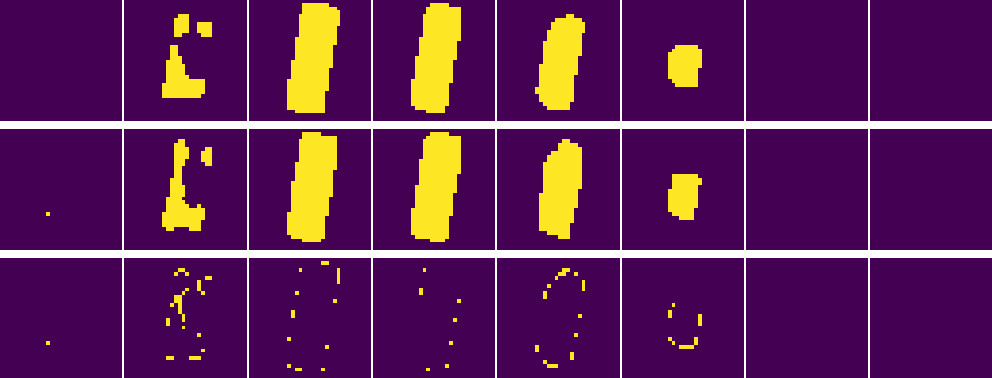
\includegraphics[width=6cm]{experiments/shapenet/vae_occ/easy_15_long/results_2}
    };
    
    \node at (6.5, 0){
      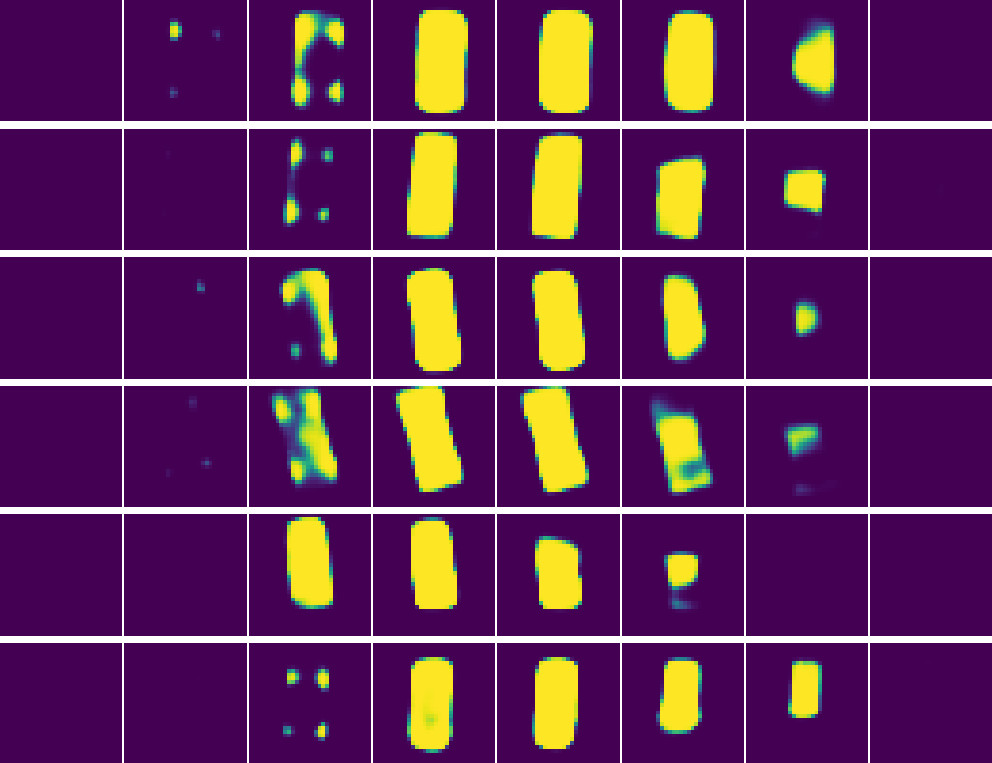
\includegraphics[width=6cm]{experiments/shapenet/vae_occ/easy_15_long/random_0}
    };
    
    \node at (0, 3) {\begin{tabular}{c}reconstruction\\occupancy\end{tabular}};
    \node at (6.5, 3) {\begin{tabular}{c}random samples\\occupancy\end{tabular}};
    
    \draw[-,dashed] (-3.5, -2.5) -- (10, -2.5);
    
    \node at (10, 0) {
      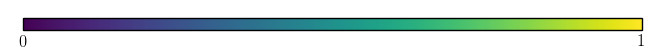
\includegraphics[height=4.2cm]{experiments/3d/vae_occ/easy_15/colorbar}
    };
    
    %\node at (-3.5,-5) {
    %  \includegraphics[height=5cm]{experiments/3d/vae_occ_sdf/colorbar_0}
    %};
    
    \node at (0, -5){
      \includegraphics[width=6cm]{experiments/shapenet/vae_occ_sdf/easy_15/random_0_0}
    };
    
    %\draw[-,dashed] (3.25, -3) -- (3.25,3);
    
    \node at (6.5, -5){
      \includegraphics[width=6cm]{experiments/shapenet/vae_occ_sdf/easy_15/random_0_1}
    };
    
    \node at (10,-5) {
      \includegraphics[height=5cm]{experiments/3d/vae_occ_sdf/colorbar_1}
    };
    
    \node[rotate=90] at (-3.75, 0) {\begin{tabular}{c}predicting occupancy only\end{tabular}};
    \node[rotate=90] at (-3.75, -5) {\begin{tabular}{c}predicting occupancy and\\signed distance functions\end{tabular}};
        
    \node at (0, -8) {\begin{tabular}{c}random samples\\occupancy\end{tabular}};
    \node at (6.5, -8) {\begin{tabular}{c}random samples\\signed distance functions\end{tabular}};
  \end{tikzpicture}
  \caption{Qualitative results considering reconstruction and random samples
  for a \VAE prior, $Q = 15$, learned on ShapeNet using occupancy only (top) and
  both occupancy and signed distance functions. In the latter case we only show
  random samples in both modalities. For reconstructions we show the target shape,
  the prediction as well as the corresponding error. In all cases we resort to
  showing horizontal slices as done before. 3D visualizations
  of the random samples can be found in Figures \ref{fig:experiments-shapenet-vae-qual-2}
  and \ref{fig:experiments-shapenet-vae-qual-3}.}
  \label{fig:experiments-shapenet-vae-qual-1}
\end{figure}
\begin{figure}
  \centering
  \hspace*{-0.75cm}
  \begin{tikzpicture}
    \node at (0, 0) {
      \includegraphics[width=2.5cm,trim={2cm 1cm 2cm 1cm},clip]{experiments/shapenet/vae_occ/easy_15_long/0_random_15}
    };
    \node at (2.5, 0) {
      \includegraphics[width=2.5cm,trim={2cm 1cm 2cm 1cm},clip]{experiments/shapenet/vae_occ/easy_15_long/0_random_105}
    };
    
    \draw[-,dashed] (4,-1.5) -- (4, 1.5);
    
    \node at (5.5, 0) {
      \includegraphics[width=2.5cm,trim={2cm 1cm 2cm 1cm},clip]{experiments/shapenet/vae_occ/easy_15_long/5_random_15}
    };
    \node at (8, 0) {
      \includegraphics[width=2.5cm,trim={2cm 1cm 2cm 1cm},clip]{experiments/shapenet/vae_occ/easy_15_long/5_random_105}
    };
    
    \draw[-,dashed] (9.5,-1.5) -- (9.5, 1.5);
    
    \node at (11, 0) {
      \includegraphics[width=2.5cm,trim={2cm 1cm 2cm 1cm},clip]{experiments/shapenet/vae_occ/easy_15_long/2_random_15}
    };
    \node at (13.5, 0) {
      \includegraphics[width=2.5cm,trim={2cm 1cm 2cm 1cm},clip]{experiments/shapenet/vae_occ/easy_15_long/2_random_105}
    };
  \end{tikzpicture}
  \caption{3D visualizations of random samples obtained from a \VAE prior
  trained with $Q = 15$ and occupancy only on the ShapeNet dataset. We show three
  distinct samples using two viewpoints each. The samples
  can easily be recognized as cars, although details seem to be missing. However,
  this is also due to the low resolution of $32^3$ used.}
  \label{fig:experiments-shapenet-vae-qual-2}
\end{figure}
\begin{figure}
  \centering
  \hspace*{-0.5cm}
  \begin{tikzpicture}   
    \node at (0, 0) {
      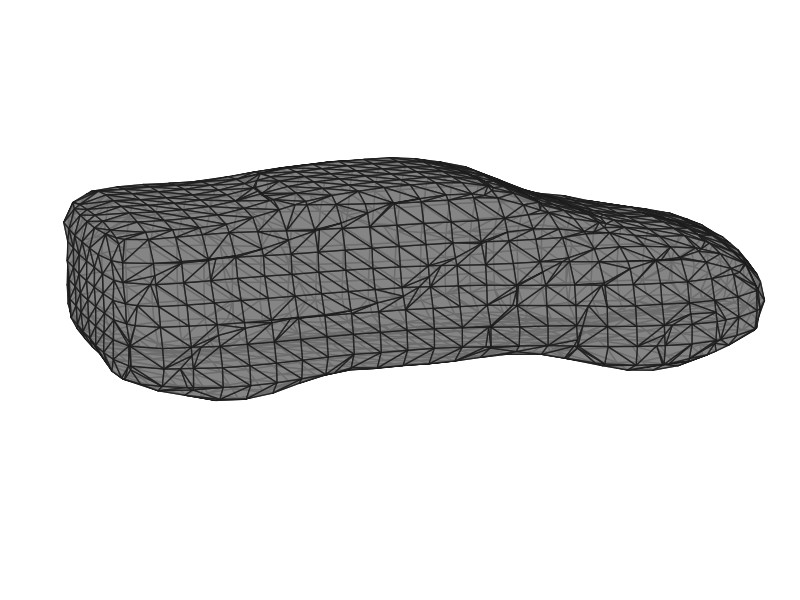
\includegraphics[width=2.4cm,trim={1cm 3cm 1cm 3cm},clip]{experiments/shapenet/vae_occ_sdf/easy_15/0_random}
    };
    
    \draw[-,dashed] (1.25,-1) -- (1.25, 1);
    
    \node at (2.5, 0) {
      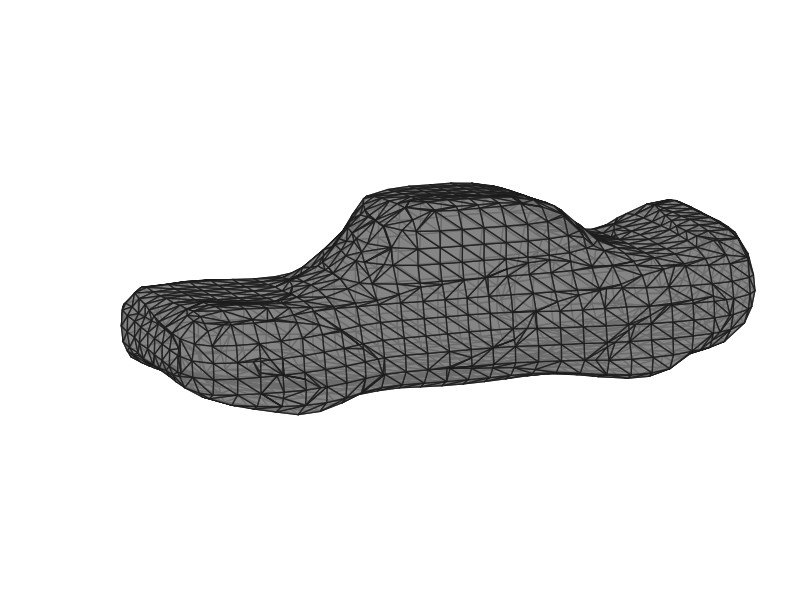
\includegraphics[width=2.4cm,trim={1cm 3cm 1cm 3cm},clip]{experiments/shapenet/vae_occ_sdf/easy_15/1_random}
    };
    
    \draw[-,dashed] (3.75,-1) -- (3.75, 1);
    
    \node at (5, 0) {
      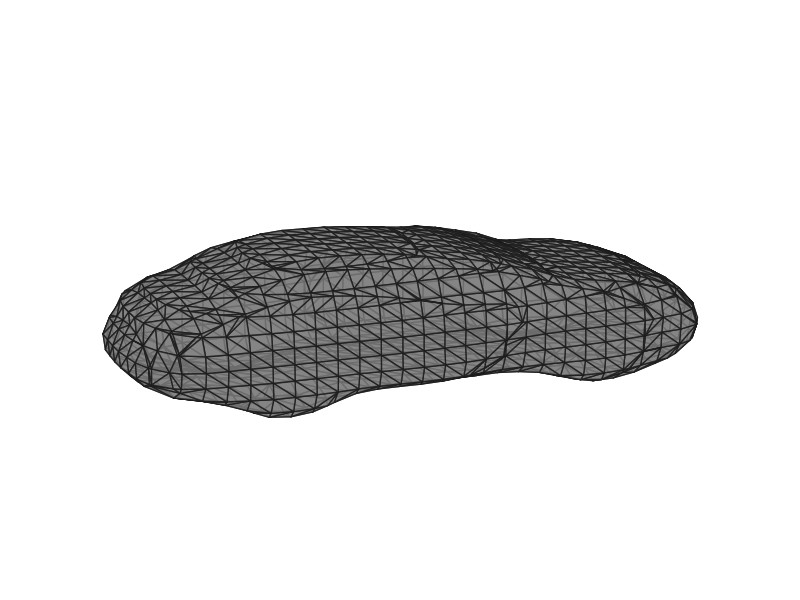
\includegraphics[width=2.4cm,trim={1cm 3cm 1cm 3cm},clip]{experiments/shapenet/vae_occ_sdf/easy_15/2_random}
    };
    
    \draw[-,dashed] (6.25,-1) -- (6.25, 1);
    
    \node at (7.5, 0) {
      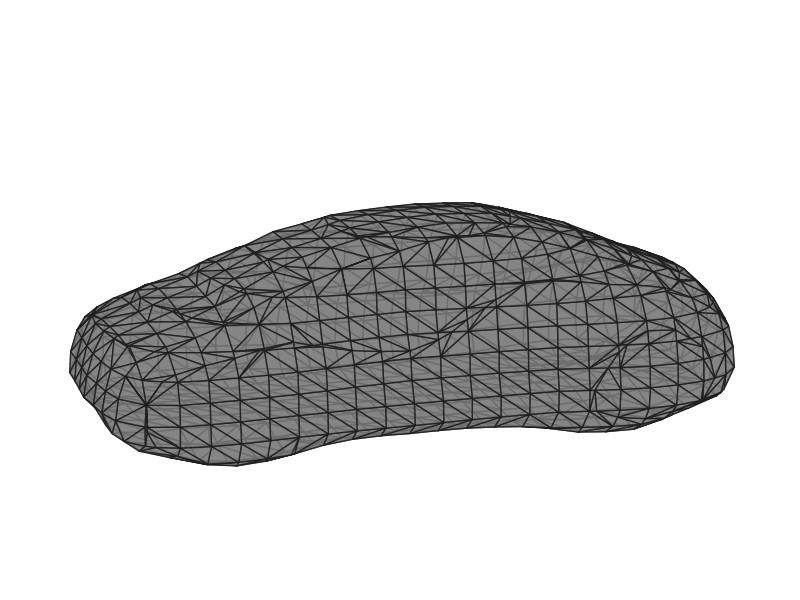
\includegraphics[width=2.4cm,trim={1cm 3cm 1cm 3cm},clip]{experiments/shapenet/vae_occ_sdf/easy_15/3_random}
    };
    
    \draw[-,dashed] (8.75,-1) -- (8.75, 1);
    
    \node at (10, 0) {
      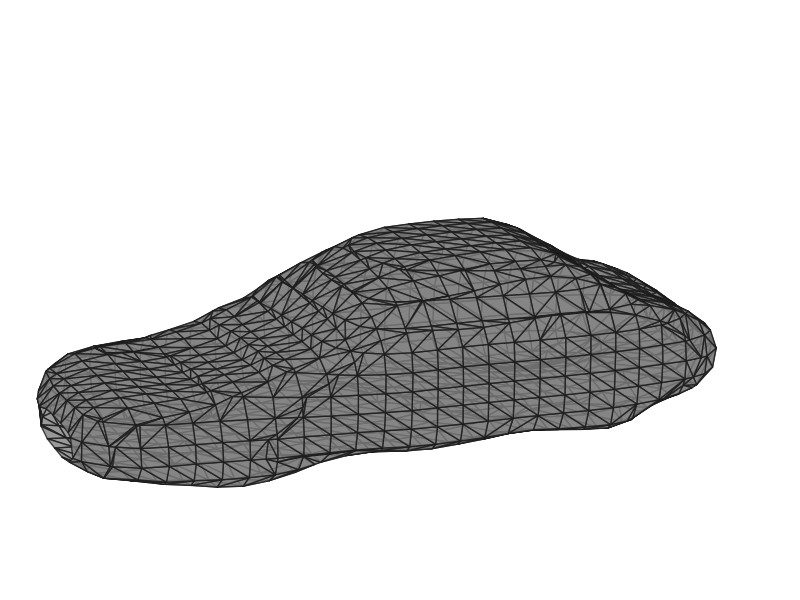
\includegraphics[width=2.4cm,trim={1cm 3cm 1cm 3cm},clip]{experiments/shapenet/vae_occ_sdf/easy_15/4_random}
    };
    
    \draw[-,dashed] (11.25,-1) -- (11.25, 1);
    
    \node at (12.5, 0) {
      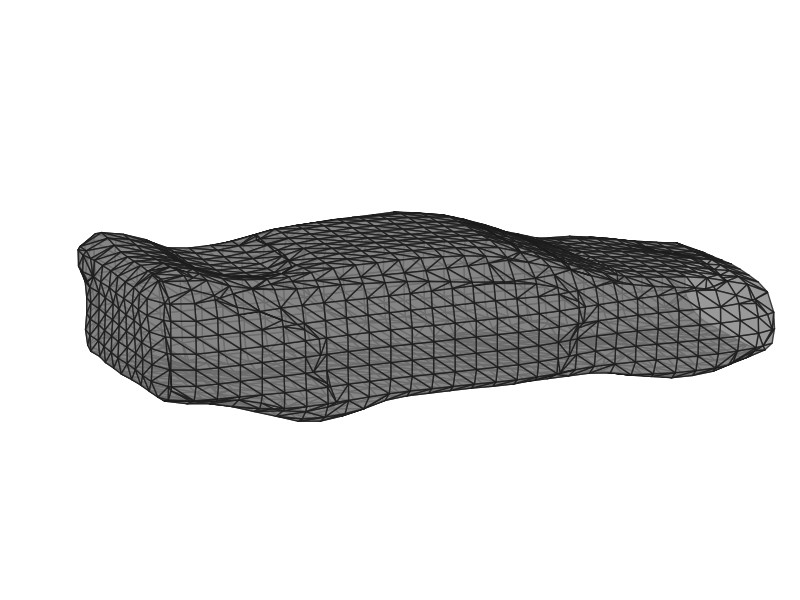
\includegraphics[width=2.4cm,trim={1cm 3cm 1cm 3cm},clip]{experiments/shapenet/vae_occ_sdf/easy_15/5_random}
    };
  \end{tikzpicture}
  \caption{3D visualizations of meshed random samples from a \VAE trained
  on both occupancy and signed distance functions. For meshing, we used the marching
  cubes algorithm on the predicted signed distance functions. We show a single viewpoint
  for each sample.}
  \label{fig:experiments-shapenet-vae-qual-3}
\end{figure}


For the \VAE prior, we again use $Q = 15$.
From training, we might conclude that the
ShapeNet dataset is slightly easier to learn. In particular, considering
Figure \ref{fig:experiments-shapenet-vae-t} we notice that both reconstruction
and the latent space are learned faster. However, it is hard to say whether
ShapeNet is inherently easier than the 3D cuboids dataset. On the one hand, we
only consider slight rotations around all axes; on the other hand,
the cars show more intra-class variation compared to cuboids. Overall,
the model achieves an absolute error of $\Abs \approx 0.0073$ and
$\AbsThr \approx 0.0048$ after thresholding.
However, we note
that only $\sim 5.54\%$ of the voxels are occupied in the first place
(\cf Table \ref{table:experiments-shapenet-datasets}).
We also notice that the model is less certain considering the random
samples in Figures \ref{fig:experiments-shapenet-vae-qual-1}
and \ref{fig:experiments-shapenet-vae-qual-2}, \ie predictions
appear less sharp. Especially regarding the wheels and the roofs, the model
has difficulties. Overall, we are satisfied by the obtained performance --
for experiments on KITTI, we will also have more training data.

On ShapeNet, too, we trained a prior model on both occupancy and signed
distance functions. For the first time, we also demonstrate why
we would prefer to work with signed distance functions: it is possible
to derive triangular meshes at sub-voxel accuracy, \eg
using the marching cubes algorithm \cite{LorensenCline:1987}\footnote{
  We use the implementation by Pablo M\'{a}rquez Neila available at
  \url{https://github.com/pmneila/PyMCubes}.
}. Again, we use $Q = 15$ to achieve a thresholded absolute error $\AbsThr \approx 0.0048$
(occupancy) and $\AbsThr \approx 0.0053$ (signed distance function), respectively.
We show meshes corresponding to random samples in Figure
\ref{fig:experiments-shapenet-vae-qual-3}. In addition,
in Figure \ref{fig:experiments-shapenet-vae-qual-1},
we show both modalities, also to illustrate the involved uncertainty.
Overall, we find that the random samples are appropriate. While some random samples
appear rather weird, it is not hard to imagine that they depict cars.
We also want to stress that the meshes look rather smooth although the
signed distance functions the model was trained on were originally derived
from the occupancy grids. We assume this to be the result of the probabilistic
formulation, \ie of training a \VAE. In particular, the encoder predicts
a Gaussian distribution where all samples need to result in a proper reconstruction.
This forces the model the smoothly interpolate between shapes.

\subsection{Amortized Maximum Likelihood}

\begin{figure}
  \centering
  \begin{tikzpicture}
    \begin{axis}[
        ybar stacked,
        % https://tex.stackexchange.com/questions/119887/remove-the-scientific-notation-which-is-unreasonable
        yticklabel style={
          /pgf/number format/fixed,
          /pgf/number format/precision=5
        },
        scaled y ticks=false,
        %enlargelimits=0.15,
        legend style={
          at={(1.01,1)},
          anchor=north west,
        },
        % https://tex.stackexchange.com/questions/48620/pgfplots-alignment-and-size-of-math-in-legend
        legend cell align=left,
        xtick={
          1, 2,
          3, 4, 5,
          6, 7, 8,
          9, 10, 11,
          12
        },
        xticklabels={
          \VAE, \VAE +sdf,
          \AML\\\easy, \AML\\\moderate, \AML\\\hard,
          \EVAE\\\easy, \EVAE\\\moderate, \EVAE\\\hard,
          \AML +sdf\\\easy, \AML +sdf\\\moderate, \AML +sdf\\\hard,
          Baseline
        },
        x tick label style={text width=1.5cm,align=right},
        ymin=0,
        width=12.5cm,
        height=4cm,
        enlarge x limits=0.05,
        % https://tex.stackexchange.com/questions/271027/pgfplots-how-to-rotate-extra-x-tick-labels
        x tick label style={
          rotate=90,
          anchor=east,
        },
        %bar width=8,
      ]
      
      % AbsThr
      \addplot +[bar shift=-.2cm] coordinates {
        (1, 0.00505722)
        (2, 0.00475067)
        (3, 0.01667228)
        (4, 0.0215971)
        (5, 0.02619364)
        %
        (6, 0.02136223)
        (7, 0.02775098)
        (8, 0.03063716)
        %
        (9, 0.02538469)
        (10, 0.03168048)
        (11, 0.03483872)
        (12, 0.010504529630079)
      };
      \addlegendentry{\AbsThr (occ)}
      % Abs
      \addplot +[bar shift=-.2cm] coordinates {
        (1, 0.002275) % 0.00733222)
        (2, 0.00203) % 0.00678092)
        (3, 0.00101) % 0.01768816)
        (4, 0.00088) % 0.02247298)
        (5, 0.00099) % 0.02718333)
        %
        (6, 0.00083) % 0.02219768)
        (7, 0.00063) % 0.02838561)
        (8, 0.0031) % 0.03373657)
        %
        (9, 0.00051) % 0.02589711)
        (10, 0.00041) % 0.0320905)
        (11, 0.00019) % 0.0350219)
        (12, 0.003366) % 0.013873896760899)
      };
      \addlegendentry{\Abs (occ)}
      
      % -- 
      \resettwelvestackedplots
      
      % AbsThr
      \addplot +[bar shift=+.2cm] coordinates {
        (1, 0)
        (2, 0.00530342)
        (3, 0)
        (4, 0)
        (5, 0)
        %
        (6, 0)
        (7, 0)
        (8, 0)
        %
        (9, 0.02553955)
        (10, 0.03210551)
        (11, 0.03564795)
        (12, 0)
      };
      \addlegendentry{\AbsThr (sdf)}
      % Abs
      \addplot +[bar shift=+.2cm] coordinates {
        (1, 0)
        (2, 0.0733) % 0.07860103)
        (3, 0)
        (4, 0)
        (5, 0)
        %
        (6, 0)
        (7, 0)
        (8, 0)
        %
        (9, 0.15607) % 0.18164451)
        (10, 0.1978) % 0.2299151)
        (11, 0.2304) % 0.26641559)
        (12, 0)
      };
      \addlegendentry{\Abs (sdf)}
    \end{axis}
  \end{tikzpicture}
  
  % TODO short caption
  \caption{Absolute error \Abs and its thresholded variant \AbsThr,
  \ie the absolute error on thresholded predictions,
  comparing \AML and \EVAE with the supervised baseline and the
  reconstruction performance of the shape prior. For the \VAE shape prior,
  we report the reconstruction performance for training on
  occupancy only as well as on both occupancy and signed distance functions.
  For \AML, we also consider both modalities. For \EVAE and the supervised baseline,
  we present results on occupancy only. For the latter, we refer to
  Section \ref{sec:experiments-shapenet-supervised-baseline}
  for details. In all cases, the left bar represents
  results on occupancy; the right bar corresponds to results on signed distance
  functions (if applicable).}
  \label{fig:experiments-shapenet-aml-abs}
\end{figure}

\begin{figure}
  \centering
  \begin{tikzpicture}    
    \node at (10, 0) {
      \includegraphics[height=4.2cm]{experiments/3d/vae_occ/easy_15/colorbar}
    };
    
    \node at (0, 0){
      \includegraphics[width=6cm]{experiments/shapenet/vae_occ_aml/hard_15_long_statistics_75/results_0}
    };
    
    \node at (6.5, 0){
      \includegraphics[width=6cm]{experiments/shapenet/vae_occ_aml/hard_15_long_statistics_75/results_3}
    };
    
    \draw[-,dashed](-3.5,-2.15) -- (10,-2.15);
    
    % --- 
    \node at (0, -3.5){
      \includegraphics[width=6cm]{experiments/shapenet/baseline/hard_15/results_0}
    };
    
    \node at (6.5, -3.5){
      \includegraphics[width=6cm]{experiments/shapenet/baseline/hard_15/results_3}
    };
    
    \node[rotate=90] at (-3.5, -3.5) {Baseline};
    \node[rotate=90] at (-3.5, 0) {\AML};
    %\node at (3.25, 2.5) {reconstruction};
  \end{tikzpicture}
  \vskip 6px
  
  % TODO short caption
  \caption{Qualitative results of \AML for \hard difficulty of the ShapeNet
  dataset. We show results for occupancy only in comparison with the supervised
  baseline. On top, we show horizontal slices of the volumes
  corresponding to the observed points, the partial free space, the target
  shape, the predicted shape and the corresponding error. On the bottom,
  \ie for the baseline, we only show the target shape, the predicted shape
  and the corresponding error. Again, we show heights $8 + 2i$ for
  $0 \leq i < 8$. 3D visualizations of these results can be found
  in Figure \ref{fig:experiments-shapenet-aml-qual-2}.}
  \label{fig:experiments-shapenet-aml-qual-1}
\end{figure}
\begin{figure}
  \centering
  \hspace*{-1cm}
  \begin{tikzpicture}
    \node at (0, 0) {
      \includegraphics[width=3.75cm,trim={3.5cm 2.5cm 3.5cm 2.5cm},clip]{experiments/shapenet/vae_occ_aml/hard_15_long_statistics_75/0_input_45}
    };
    \node at (3.5, 0) {
      \includegraphics[width=3.75cm,trim={3.5cm 2.5cm 3.5cm 2.5cm},clip]{experiments/shapenet/vae_occ_aml/hard_15_long_statistics_75/0_prediction_45}
    };
    \node at (7, 0) {
      \includegraphics[width=3.75cm,trim={3.5cm 2.5cm 3.5cm 2.5cm},clip]{experiments/shapenet/vae_occ_aml/hard_15_long_statistics_75/0_target_45}
    };
    \node at (10.5, 0) {
      \includegraphics[width=3.75cm,trim={3.5cm 2.5cm 3.5cm 2.5cm},clip]{experiments/shapenet/baseline/hard_15/0_prediction_45}
    };
    
    \node at (0, -3) {
      \includegraphics[width=3.75cm,trim={3.5cm 2.5cm 3.5cm 2.5cm},clip]{experiments/shapenet/vae_occ_aml/hard_15_long_statistics_75/3_input_45}
    };
    \node at (3.5, -3) {
      \includegraphics[width=3.75cm,trim={3.5cm 2.5cm 3.5cm 2.5cm},clip]{experiments/shapenet/vae_occ_aml/hard_15_long_statistics_75/3_prediction_45}
    };
    \node at (7, -3) {
      \includegraphics[width=3.75cm,trim={3.5cm 2.5cm 3.5cm 2.5cm},clip]{experiments/shapenet/vae_occ_aml/hard_15_long_statistics_75/3_target_45}
    };
    \node at (10.5, -3) {
      \includegraphics[width=3.75cm,trim={3.5cm 2.5cm 3.5cm 2.5cm},clip]{experiments/shapenet/baseline/hard_15/3_prediction_45}
    };
    
    \node at (0, 1.75) {Input};
    \node at (3.5, 1.75) {\AML};
    \node at (7, 1.75) {Baseline};
    \node at (10.5, 1.75) {Target};
  \end{tikzpicture}
  \caption{3D visualizations for comparing \AML and the supervised baseline
  on \hard difficulty of the ShapeNet dataset. Results were obtained using occupancy
  only. As can be seen, \AML has difficulties with the roofs; additionally,
  the first example occurs to the predicted with flipped orientation as our
  ShapeNet dataset also includes flipped variants.}
  \label{fig:experiments-shapenet-aml-qual-2}
\end{figure}
\begin{figure}
  \centering
  \begin{tikzpicture}    
    \node at (-3.5,0) {
      \includegraphics[height=4.25cm]{experiments/3d/vae_occ_sdf/colorbar_0}
    };
    
    \node at (0, 0){
      \includegraphics[width=6cm]{experiments/shapenet/vae_occ_sdf_aml/hard_15_statistics/results_0_0}
    };
    \node at (0, -4){
      \includegraphics[width=6cm]{experiments/shapenet/vae_occ_sdf_aml/hard_15_statistics/results_3_0}
    };
    
    \node at (6.5, 0){
      \includegraphics[width=6cm]{experiments/shapenet/vae_occ_sdf_aml/hard_15_statistics/results_0_1}
    };
    \node at (6.5, -4){
      \includegraphics[width=6cm]{experiments/shapenet/vae_occ_sdf_aml/hard_15_statistics/results_3_1}
    };
    
    \node at (10,0) {
      \includegraphics[height=4.25cm]{experiments/3d/vae_occ_sdf/colorbar_1}
    };
    
    \node at (0, 2.25) {occupancy};
    \node at (6.5, 2.25) {signed distance function};
  \end{tikzpicture}
  \vskip 6px

  % TODO short caption
  \caption{Qualitative results for \AML using both occupancy and signed distance
  functions. We show two examples from the \hard dataset for both modalities.
  In both cases we show slices of the volumes corresponding to the observed points,
  the partial free space, the target shape as well as the predicted shape and its
  error. Again, we show heights $8 + 2i$ for $0 \leq i < 8$. Triangular meshes
  corresponding the the predicted signed distance functions can be found
  in Figure \ref{fig:experiments-shapenet-aml-qual-4}.}
  \label{fig:experiments-shapenet-aml-qual-3}
\end{figure}
\begin{figure}
  \centering
  \begin{tikzpicture}
    \node at (0, 0) {
      \includegraphics[width=2.75cm,trim={1cm 2cm 1cm 2cm},clip]{experiments/shapenet/vae_occ_sdf_aml/hard_15_statistics/0_prediction}
    };
    \node at (3, 0) {
      \includegraphics[width=2.75cm,trim={1cm 2cm 1cm 2cm},clip]{experiments/shapenet/vae_occ_sdf_aml/hard_15_statistics/0_target}
    };
    
    \draw[-,dashed] (5,-1) -- (5, 1);
    
    \node at (7, 0) {
      \includegraphics[width=2.75cm,trim={1cm 2cm 1cm 2cm},clip]{experiments/shapenet/vae_occ_sdf_aml/hard_15_statistics/3_prediction}
    };
    \node at (10, 0) {
      \includegraphics[width=2.75cm,trim={1cm 2cm 1cm 2cm},clip]{experiments/shapenet/vae_occ_sdf_aml/hard_15_statistics/3_target}
    };
    
    \node at (0, 1) {\AML};
    \node at (3, 1) {Target};
    \node at (7, 1) {\AML};
    \node at (10, 1) {Target};
  \end{tikzpicture}
  \caption{Qualitative results for \AML after using marchign cubes to
  derive meshes from the predictions and the targets. For the targets, we can
  clearly see that the used signed distance functions are derived from the
  occupancy grids. The predictions, in contrast a re more smooth, however,
  consistently underestimate the size of the car.}
  \label{fig:experiments-shapenet-aml-qual-4}
\end{figure}


% TODO zero error in all plots
For \AML, we follow the procedure of the 3D cuboids dataset; in Figure
\ref{fig:experiments-shapenet-aml-abs} we plot
quantitative results for the \easy, \moderate and \hard cases.
Again, it is important to keep in mind that only roughly $5.54\%$ of the voxels
are occupied. Thus, results for the \moderate and \hard cases seem quite poor:
$\Abs \approx 0.023$ and $\Abs \approx 0.027$, respectively.
This can also be observed when considering qualitative results in
Figures \ref{fig:experiments-shapenet-aml-qual-1} and
\ref{fig:experiments-shapenet-aml-qual-2} showing results for the \hard case.
We found that in many case, the predictions are very uncertain.
When considering 3D visualizations this is stressed even
more due to the thresholding. For the \moderate case, in contrast, results
look more plausible in many cases. We are not sure whether these
observations can be attributed to the prior model -- which could \eg
not be trained long enough -- or the variation in the dataset that allows
these models. It might also be beneficial to enforce the negative log-likelihood
on the prior $p(z)$ more stringent -- this assumes that the latent space
is ``more reliable'' close to $0$ than towards the tail of the Gaussian.
This could prevent shape inference from learning unlikely shapes and
potentially reduce the influence of weight initialization and stochastic
training in the first few epochs.
Overall, we see potential for improvement by tuning hyper-parameters and
longer training.

When predicting both occupancy and signed distance functions, we are not able
to achieve a performance comparable to the occupancy only case. Especially
in the \moderate and \hard cases, performance drops significantly from
$\Abs \approx 0.026$ to $\Abs \approx 0.032$ or higher (on occupancy).
We cannot say whether this is a drawback of
signed distance functions as modality, due to the shape prior or because of
the training procedure. In contrast to the occupancy only case, we did not
spend as much time tuning parameters. An exact comparison can be found in 
Figure \ref{fig:experiments-shapenet-aml-abs} while we show qualitative
results in Figures \ref{fig:experiments-shapenet-aml-qual-3}
and \ref{fig:experiments-shapenet-aml-qual-4}.
Considering the qualitative results we can, however, appreciate the
smoothing effect on the prior; the meshed predictions look very appealing -- 
in contrast to the meshed targets. Here it gets apparent that our signed
distance functions are derived from the occupancy grids. We can also
see the drop in performance; some predictions do not match the targets as
well as before; especially as \AML consistently underestimates the size
of the cars. The problems with predicting signed distance functions seem
to be consistent across datasets and models; overall, we believe that
an alternative representation might be easier to learn, \eg normalized,
discretized or just replacing the logarithm.

\subsection{Extended Variational Auto Encoder}

Although \EVAE performed slightly worse than \AML on the 3D cuboids dataset,
we still include quantitative results in Figure \ref{fig:experiments-shapenet-aml-abs}.
On ShapeNet, the performance difference between \AML and \EVAE becomes more pronounced.
However, we also want to note that, again, we did not put as much effort into
tuning parameters and training compared to \AML. Specifically, we suspect that
the weight on the Kullback-Leibler divergences may make a significant
difference. Unfortunately, we were unable to investigate this problem
further. Still, we showed, that the framework is also applicable to
real-world objects -- even if only the \easy case results in appropriate performance.
%We provide
%qualitative results in the appendix.

\subsection{Supervised Baseline}
\label{sec:experiments-shapenet-supervised-baseline}

For ShapeNet, we also prepared a supervised baseline. For a fair comparison,
we used the shape prior architecture with $Q = 15$, to learn the mapping
$x_n \mapsto y_n^*$ directly from the
synthetic data. We did not notice a significant difference between training the
exact same architecture versus removing the
Kullback-Leibler divergence and the corresponding reparameterization layer; for fairness,
we followed the former approach. We considered the \hard case only. Later,
we will also evaluate how well the learned model generalizes to KITTI.
Figure \ref{fig:experiments-shapenet-aml-abs}
shows that supervision is able to get closer to the reconstruction performance
of the shape prior, with an
absolute error of roughly $\Abs \approx 0.014$ thereby outperforming all other
presented approaches for shape completion. Qualitative results are shown in Figures
\ref{fig:experiments-shapenet-aml-qual-1} and \ref{fig:experiments-shapenet-aml-qual-2}
in comparison with \AML. Overall,
the supervised baseline could potentially also outperform \AML on KITTI, given
that the used observation model resembles KITTI's Velodyne sensor closely
enough. Overall, it is not surprising that the supervised baseline outperforms
\AML considering that \AML only uses a fraction, in particular $4.06\%$ in the
\moderate case, of the information during training.

\subsection{Discussion}

Overall, the results obtained on ShapeNet are not convincing in all cases. Especially
on \moderate and \hard difficulty, shape completion appears to be significantly
more challenging than on the 3D cuboids dataset. Unfortunately, limited time prevented us
from conducting more experiments regarding both prior and shape completion, \eg to investigate
the influence of training time, architectural changes and hyper-parameters. 
Still, the presented experiments show that the proposed approach, especially \AML
but also \EVAE in a limited setting,
are able to learn shape completion under difficult conditions.
Although we were not able to reach supervised performance, it is still surprising
what is possible under weak supervision when relying on strong shape priors.
%On KITTI,
%we also hope that a larger training set for the prior (\ie both training sets from
%Table \ref{table:experiments-shapenet-datasets}) will improve results.
We discuss possible future experiments
based on the above observations in detail in in Section \ref{sec:future-work}.

\section{KITTI}

Using ShapeNet \cite{ChangFunkhouserGuibasSavarese:2015} we are able to learn
a shape prior enabling us to perform shape completion on KITTI
\cite{GeigerLenzUrtasun:2012,GeigerLenzStillerUrtasun:2013}.
On KITTI, however, we do not have access to ground truth shapes.
We found that manual annotation (\eg following \cite{MenzeGeiger:2015}) 
would go far beyond the time frame of this thesis. Still,
we intend to provide insightful experiments thereby, again, focusing on
\AML using both modalities, \ie occupancy and signed distance functions.
Our goal is to demonstrate that \AML is able to predict reasonable
shapes given the noisy observations from KITTI's Velodyne sensor.

Following the discussion in Section \ref{sec:data-kitti}, we filtered
the provided ground truth 3D bounding boxes using $n_{1,\min} = 150$,
$n_{0,\min} = 1500$ and $t_{\max} = 30$. This means, that we require at least
$150$ voxels to be observed as occupied and $1500$ observed voxels
to correspond to free space. Additionally, we only consider bounding boxes
within $30m$ of the sensor. Overall, we obtained $1928$ distinct car observations
which we split into a training set with $1714$ and a validation with
$214$ samples.
On average, $\sim 0.634\%$ of voxels are observed points; $\sim 5.98\%$
of voxels are free space. In this regard, the dataset might be slightly
easier than the \hard ShapeNet dataset, where only $0.304\%$ of voxels are
observed as being occupied. In spite of these strict requirements regarding
the number of observed voxels, we find the extracted dataset to be particularly
challenging due to the corresponding noise patterns. We show additional examples
of the dataset in Appendix \ref{ch:appendix-data}.
% TODO examples!

\subsection{Amortized Maximum Likelihood}

\begin{figure}
  \centering
  \begin{tikzpicture}
    \node at (0, 0){
      \includegraphics[width=6cm]{experiments/kitti/vae_occ_aml/15_long/results_1}
    };
    \node at (0, -2.5){
      \includegraphics[width=6cm]{experiments/kitti/vae_occ_aml/15_long_statistics/results_1}
    };
    \node at (0, -5){
      \includegraphics[width=6cm]{experiments/kitti/vae_occ_aml/15_long_statistics_combined/results_1}
    };
   
    \node at (6.25, 0){
      \includegraphics[width=6cm]{experiments/kitti/vae_occ_aml/15_long/results_4}
    };
    \node at (6.25, -2.5){
      \includegraphics[width=6cm]{experiments/kitti/vae_occ_aml/15_long_statistics/results_4}
    };
    \node at (6.25, -5){
      \includegraphics[width=6cm]{experiments/kitti/vae_occ_aml/15_long_statistics_combined/results_4}
    };
    
    \draw[-,dashed] (-3.25, -1.25) -- (9.5,-1.25);
    \draw[-,dashed] (-3.25, -3.75) -- (9.5,-3.75);
    
    %\node at (10,0) {
    %  \includegraphics[height=2.5cm]{experiments/3d/vae_occ/easy_15/colorbar}
    %};
    
    \node at (3.25, 1.5) {reconstruction};
    \node[rotate=90] at (-3.5, 0) {\AML};
    \node[rotate=90] at (-3.75, -2.5) {\begin{tabular}{c}\AML\\+weights\end{tabular}};
    \node[rotate=90] at (-4, -5) {\begin{tabular}{c}\AML\\+weights\\+combined\end{tabular}};
  \end{tikzpicture}

  % TODO short caption
  \caption{Qualitative results for \AML on the extracted KITTI dataset. We demonstrate
  the influence of using the weights $\rho_i$ marked as +weights; here, the weights are
  pre-computed on ShapeNet as discussed for Equation \eqref{eq:experiments-3d-weights}.
  Additionally we show the influence of training the prior on both ShapeNet training sets,
  referred to as +combined. As always, we show horizontal slices for the observed points,
  the corresponding partial free space and the predictions.
  }
  \label{fig:experiments-kitti-aml-1}
\end{figure}

\begin{figure}
  \centering
  %\hspace*{-1.5cm}
  \begin{tikzpicture}
    \node at (0, 0) {
      \includegraphics[width=3.75cm,trim={3.5cm 2.5cm 3.5cm 2.5cm},clip]{experiments/kitti/vae_occ_aml/15_long_statistics_combined/0_input_45}
    };
    \node at (3.5, 0) {
      \includegraphics[width=3.75cm,trim={3.5cm 2.5cm 3.5cm 2.5cm},clip]{experiments/kitti/vae_occ_aml/15_long_statistics_combined/0_prediction_45}
    };
    \node at (7, 0) {
      \includegraphics[width=3.75cm,trim={3.5cm 2.5cm 3.5cm 2.5cm},clip]{experiments/kitti/baseline/moderate_15/0_prediction_45}
    };

    % \node at (7, 0) {
    %   \includegraphics[width=3.75cm,trim={3.5cm 2.5cm 3.5cm 2.5cm},clip]{experiments/kitti/vae_occ_aml/15_long_statistics_combined/2_input_135}
    % };
    % \node at (10.5, 0) {
    %   \includegraphics[width=3.75cm,trim={3.5cm 2.5cm 3.5cm 2.5cm},clip]{experiments/kitti/vae_occ_aml/15_long_statistics_combined/2_prediction_135}
    % };
    
    \node at (0, -3) {
      \includegraphics[width=3.75cm,trim={3.5cm 2.5cm 3.5cm 2.5cm},clip]{experiments/kitti/vae_occ_aml/15_long_statistics_combined/1_input_45}
    };
    \node at (3.5, -3) {
      \includegraphics[width=3.75cm,trim={3.5cm 2.5cm 3.5cm 2.5cm},clip]{experiments/kitti/vae_occ_aml/15_long_statistics_combined/1_prediction_45}
    };
    \node at (7, -3) {
      \includegraphics[width=3.75cm,trim={3.5cm 2.5cm 3.5cm 2.5cm},clip]{experiments/kitti/baseline/moderate_15/1_prediction_45}
    };

    % \node at (7, -3) {
    %   \includegraphics[width=3.75cm,trim={3.5cm 2.5cm 3.5cm 2.5cm},clip]{experiments/kitti/vae_occ_aml/15_long_statistics_combined/0_input_135}
    % };
    % \node at (10.5, -3) {
    %   \includegraphics[width=3.75cm,trim={3.5cm 2.5cm 3.5cm 2.5cm},clip]{experiments/kitti/vae_occ_aml/15_long_statistics_combined/0_prediction_135}
    % };
  
    \node at (0, -6) {
      \includegraphics[width=3.75cm,trim={3.5cm 2.5cm 3.5cm 2.5cm},clip]{experiments/kitti/vae_occ_aml/15_long_statistics_combined/2_input_45}
    };
    \node at (3.5, -6) {
      \includegraphics[width=3.75cm,trim={3.5cm 2.5cm 3.5cm 2.5cm},clip]{experiments/kitti/vae_occ_aml/15_long_statistics_combined/2_prediction_45}
    };
    \node at (7, -6) {
      \includegraphics[width=3.75cm,trim={3.5cm 2.5cm 3.5cm 2.5cm},clip]{experiments/kitti/baseline/moderate_15/2_prediction_45}
    };

    % \node at (7, -6) {
    %   \includegraphics[width=3.75cm,trim={3.5cm 2.5cm 3.5cm 2.5cm},clip]{experiments/kitti/vae_occ_aml/15_long_statistics_combined/1_input_135}
    % };
    % \node at (10.5, -6) {
    %   \includegraphics[width=3.75cm,trim={3.5cm 2.5cm 3.5cm 2.5cm},clip]{experiments/kitti/vae_occ_aml/15_long_statistics_combined/1_prediction_135}
    % };
    
    \node at (0, -9) {
      \includegraphics[width=3.75cm,trim={3.5cm 2.5cm 3.5cm 2.5cm},clip]{experiments/kitti/vae_occ_aml/15_long_statistics_combined/3_input_45}
    };
    \node at (3.5, -9) {
      \includegraphics[width=3.75cm,trim={3.5cm 2.5cm 3.5cm 2.5cm},clip]{experiments/kitti/vae_occ_aml/15_long_statistics_combined/3_prediction_45}
    };
    \node at (7, -9) {
      \includegraphics[width=3.75cm,trim={3.5cm 2.5cm 3.5cm 2.5cm},clip]{experiments/kitti/baseline/moderate_15/3_prediction_45}
    };

    % \node at (7, -9) {
    %   \includegraphics[width=3.75cm,trim={3.5cm 2.5cm 3.5cm 2.5cm},clip]{experiments/kitti/vae_occ_aml/15_long_statistics_combined/4_input_135}
    % };
    % \node at (10.5, -9) {
    %   \includegraphics[width=3.75cm,trim={3.5cm 2.5cm 3.5cm 2.5cm},clip]{experiments/kitti/vae_occ_aml/15_long_statistics_combined/4_prediction_135}
    % };
    
    \node at (0, -12) {
      \includegraphics[width=3.75cm,trim={3.5cm 2.5cm 3.5cm 2.5cm},clip]{experiments/kitti/vae_occ_aml/15_long_statistics_combined/4_input_45}
    };
    \node at (3.5, -12) {
      \includegraphics[width=3.75cm,trim={3.5cm 2.5cm 3.5cm 2.5cm},clip]{experiments/kitti/vae_occ_aml/15_long_statistics_combined/4_prediction_45}
    };
    \node at (7, -12) {
      \includegraphics[width=3.75cm,trim={3.5cm 2.5cm 3.5cm 2.5cm},clip]{experiments/kitti/baseline/moderate_15/4_prediction_45}
    };

    \node at (0, 1.75) {Input};
    \node at (3.5, 1.75) {\AML};
    \node at (7, 1.75) {Baseline};
  \end{tikzpicture}

  % TODO short caption
  \caption{Comparison of \AML and the supervised baseline on KITTI; here,
  \AML uses occupancy only and we show the observed points and the predicted shapes
  in voxelized form. For both, we show 2 distinct viewpoints. For \AML we show
  two examples. For the latter, we also show the predicted shape using the supervised
  baseline to illustrate that \AML still misses details, \eg along the root.}
  \label{fig:experiments-kitti-aml-2}
\end{figure}
\begin{figure}
  \centering
  \begin{tikzpicture}
    \node at (0, 0) {
      \includegraphics[width=3.75cm,trim={3.5cm 2.5cm 3.5cm 2.5cm},clip]{experiments/kitti/vae_occ_sdf_aml/15_statistics_combined_075/0_input_45}
    };
    \node at (3.5, 0) {
      \includegraphics[width=3.75cm,trim={3.5cm 2.5cm 3.5cm 2.5cm},clip]{experiments/kitti/vae_occ_sdf_aml/15_statistics_combined_075/0_prediction_45}
    };
    \node at (8, 0) {
      \includegraphics[width=3.75cm,trim={1cm 3cm 1cm 3cm},clip]{experiments/kitti/vae_occ_sdf_aml/15_statistics_combined_075/0_prediction}
    };
    
    \node at (0, -3) {
      \includegraphics[width=3.75cm,trim={3.5cm 2.5cm 3.5cm 2.5cm},clip]{experiments/kitti/vae_occ_sdf_aml/15_statistics_combined_075/1_input_45}
    };
    \node at (3.5, -3) {
      \includegraphics[width=3.75cm,trim={3.5cm 2.5cm 3.5cm 2.5cm},clip]{experiments/kitti/vae_occ_sdf_aml/15_statistics_combined_075/1_prediction_45}
    };
    \node at (8, -3) {
      \includegraphics[width=3.75cm,trim={1cm 3cm 1cm 3cm},clip]{experiments/kitti/vae_occ_sdf_aml/15_statistics_combined_075/1_prediction}
    };

    \node at (0, -3) {
      \includegraphics[width=3.75cm,trim={3.5cm 2.5cm 3.5cm 2.5cm},clip]{experiments/kitti/vae_occ_sdf_aml/15_statistics_combined_075/2_input_45}
    };
    \node at (3.5, -3) {
      \includegraphics[width=3.75cm,trim={3.5cm 2.5cm 3.5cm 2.5cm},clip]{experiments/kitti/vae_occ_sdf_aml/15_statistics_combined_075/2_prediction_45}
    };
    \node at (8, -3) {
      \includegraphics[width=3.75cm,trim={1cm 3cm 1cm 3cm},clip]{experiments/kitti/vae_occ_sdf_aml/15_statistics_combined_075/2_prediction}
    };
    
    \node at (0, 1.85) {input};
    \node at (3.5, 1.85) {prediction};
    \node at (8, 1.85) {mesh};
  \end{tikzpicture}

  % TODO short caption
  \caption{3D vsualizations of the predicted shapes using \AML predicting
  both occupancy and signed distance functions. The meshes on the right
  were derived using marching cubes.}
  \label{fig:experiments-kitti-aml-3}
\end{figure}


Using \AML, we are able to obtain reasonable shape completions from the
noisy observations. As shape prior, we re-trained the model used for ShapeNet
on all $40992$ samples from both training sets, \cf Table
\ref{table:experiments-shapenet-datasets}. In Figure
\ref{fig:experiments-kitti-aml-1} we first show
the observations, \ie observed points and free space, together with
the shape predictions for several examples from the validation set.
We also show the influence of using the weights from Equation
\eqref{eq:experiments-3d-weights} as well as training the prior on the combined
ShapeNet training sets.
As expected, using the weighted
loss has significant influence on the quality of the predicted shapes. In addition,
we also notice the benefit of having more training data for the prior. For the remaining
discussion we always use the weights as well as the stronger prior.
In Figure \ref{fig:experiments-kitti-aml-2} we show 3D visualizations
corresponding to the voxelized observations and the predicted shapes.
We find that the predicted shapes match the observed points rather well
and clearly depict cars. However, the predictions still miss a considerable
level of detail around the wheels and the roof. This can be seen as the
trade-off between noise robustness,
integrated through a strong prior, and detail-orientation.
Surprisingly, the predicted shapes look better than on the \hard ShapeNet-based
dataset, \ie Figure \ref{fig:experiments-shapenet-aml-qual-2}. This confirms our
intuition that the observations extracted from KITTI are slightly easier.
%In the conclusion, specifically Figure \ref{fig:conclusion}, we also show that
%the predicted shapes with the original scene reasonably well.
Overall, \AML is able to correctly predict orientation and rough shape
of the observed cars but also leaves room for improvement regarding details.

We also used a ShapeNet prior trained on both occupancy and signed distance
functions. However, we found the results to be slightly worse compared to
ShapeNet. As before, we suspect that longer training times and fine-tuning the
hyper parameters would be necessary to improve results. Nevertheless,
Figure \ref{fig:experiments-kitti-aml-3}
shows some examples of the predictions both in the form of occupancy grids
and meshes. As in the \hard case on ShapeNet, the prior
seems to favor small and thin cars. This tendency is emphasized by
the meshes derived using marching cubes and might be explained
by the uncertainty involved when reconstructing details such as wheels and roof.
Again, we can conclude that signed
distance functions, while being advantageous for deriving meshes, are more
difficult to learn in a weakly-supervised setting.

\subsection{Supervised Baseline}

We also investigated to which extent the supervised baseline from Section
\ref{sec:experiments-shapenet-supervised-baseline} is able to generalize to KITTI.
Figure \ref{fig:experiments-kitti-aml-2} shows qualitative results when
applying the learned model to KITTI observations. As can be seen, the model
predicts reasonable cars. In contrast to \AML,
the supervised model has no troubles predicting details along or the roof
or wheels. For some samples, however,
the predictions look very similar. Overall, the supervised baseline
appears to predict slightly more coherent shapes; but an exact evaluation and
comparison is not possible without ground truth annotations.
Overall, we find that there does not seem to be a significant gap between
\AML and the supervised baseline in terms of the visual quality of
the corresponding predictions.

\subsection{Discussion}

In the end, we can conclude that \AML is able to perform shape completion even under
real conditions as illustrated on KITTI. We also found that the supervised baseline
generalizes surprisingly well. However, compared to the supervised baseline,
\AML requires significantly less supervision. We find that using occupancy grids only,
we are able to recover slightly more detail compared to signed distance functions
as shape representation. The latter, however, allows to derive comparably smooth
meshes. As discussed before, we were not able to explore the full design space
regarding architectures, hyper-parameters and training. We expect \AML
using signed distance functions to show improved performance with increased
training time and optimized hyper parameters; however, we can only leave these
experiments for future work. Additionally, we could only judge results
qualitatively. While quantitative results are provided for ShapeNet, we do not
believe that these can be transferred one-to-one to KITTI. In particular,
we think the observation model used for ShapeNet does not completely match the true
observation model underlying KITTI. In conclusion, we are satisfied by the
demonstrated shape completion performance on KITTI and are looking forward to
future experiments in order to improve the proposed approach.


